%%%%%%%%%%%%%%%%%%%%%%%%%%%%%%%%%%%%%%%%%%%%%%%%%%%%%%%%%%%%%%%%%%%%%%%%%%%%%%%%
%% BAKALÁRSKA PRÁCA                                                           %%
%%                                                                            %%
%% Názov (sk): Algoritmy detekcie a korekcie lokálnych                        %%
%%             znehodnotení digitálneho audio signálu                         %%
%% Názov (en): Algorithms for Detection and Correction of Local               %%
%%             Degradations in Digital Audio Signals                          %%
%%                                                                            %%
%% Autor: Jakub Kúdela                                                        %%
%% Vedúci: Mgr. Daniel Toropila                                               %%
%%                                                                            %%
%% Akademický rok: 2011/2012                                                  %%
%%%%%%%%%%%%%%%%%%%%%%%%%%%%%%%%%%%%%%%%%%%%%%%%%%%%%%%%%%%%%%%%%%%%%%%%%%%%%%%%

\documentclass[12pt,a4paper]{report}
\setlength\textwidth{145mm}
\setlength\textheight{247mm}
\setlength\oddsidemargin{15mm}
\setlength\evensidemargin{15mm}
\setlength\topmargin{0mm}
\setlength\headsep{0mm}
\setlength\headheight{0mm}
\let\openright=\clearpage

% \documentclass[12pt,a4paper,twoside,openright]{report}
% \setlength\textwidth{145mm}
% \setlength\textheight{247mm}
% \setlength\oddsidemargin{15mm}
% \setlength\evensidemargin{0mm}
% \setlength\topmargin{0mm}
% \setlength\headsep{0mm}
% \setlength\headheight{0mm}
% \let\openright=\cleardoublepage


\usepackage[utf8]{inputenc}

\usepackage[english,slovak]{babel}

\usepackage{aeguill}

\usepackage{graphicx}

\usepackage{epstopdf}

\usepackage{amsmath}
\usepackage{amsthm}
\usepackage{amssymb}
\usepackage{amsfonts}

\usepackage{cmap}

\usepackage{url}


\usepackage{listings}
\usepackage{xcolor}

\definecolor{dkgreen}{rgb}{0,0.6,0}
\definecolor{gray}{rgb}{0.5,0.5,0.5}
\definecolor{mauve}{rgb}{0.58,0,0.82}

\renewcommand{\lstlistingname}{Kód}
\lstdefinestyle{sharpc}{language=[Sharp]C, frame=lr, rulecolor=\color{blue!80!black}}

\lstset{frame=tb,
  language=[Sharp]C,
  aboveskip=5mm,
  belowskip=5mm,
  showstringspaces=false,
  columns=flexible,
  basicstyle={\scriptsize\ttfamily},
  numbers=none,
  numberstyle=\tiny\color{gray},
  keywordstyle=\color{blue},
  commentstyle=\color{dkgreen},
  stringstyle=\color{mauve},
  breaklines=true,
  breakatwhitespace=true,
  tabsize=3,
}


\newcommand{\chapwithtoc}[1]{
	\chapter*{#1}
	\addcontentsline{toc}{chapter}{#1}
}

\newcommand{\secwithtoc}[1]{
	\section*{#1}
	\addcontentsline{toc}{section}{#1}
}


\begin{document}

\selectlanguage{slovak}
\frenchspacing


%\title{Algoritmy detekcie a korekcie lokálnych znehodnotení digitálneho audio signálu}
%\author{Jakub Kúdela}
%\maketitle


%%%%%%%%%%%%%%%%%%%%%%%%%%%%%%%%%%%%%%%%%%%%%%%%%%%%%%%%%%%%%%%%%%%%%%%%%%%%%%%%
%% BAKALÁRSKA PRÁCA                                                           %%
%%                                                                            %%
%% Názov (sk): Algoritmy detekcie a korekcie lokálnych                        %%
%%             znehodnotení digitálneho audio signálu                         %%
%% Názov (en): Algorithms for Detection and Correction of Local               %%
%%             Degradations in Digital Audio Signals                          %%
%%                                                                            %%
%% Autor: Jakub Kúdela                                                        %%
%% Vedúci: Mgr. Daniel Toropila                                               %%
%%                                                                            %%
%% Akademický rok: 2011/2012                                                  %%
%%%%%%%%%%%%%%%%%%%%%%%%%%%%%%%%%%%%%%%%%%%%%%%%%%%%%%%%%%%%%%%%%%%%%%%%%%%%%%%%

\begin{titlepage}
\begin{center}

\large
Univerzita Karlova v Praze

\medskip

Matematicko-fyzikální fakulta

\vfill

{\Large \textbf{BALALÁRSKA PRÁCA}}

\vfill

\includegraphics[width=60mm]{images/mff_logo.eps}

\vfill
\vspace{5mm}

{\LARGE Jakub Kúdela}

\vspace{15mm}

{\LARGE \textbf{Algoritmy detekcie a korekcie lokálnych znehodnotení digitálneho audio signálu}}

\vfill

Katedra teoretické informatiky a matematické logiky

\vfill

\begin{tabular}{rl}
Vedúci bakalárskej práce: & Mgr. Daniel Toropila\\
\noalign{\vspace{2mm}}
Študijný program: & Informatika\\
\noalign{\vspace{2mm}}
Študijný odbor: & Teoretická informatika\\
\end{tabular}

\vfill

Praha 2012

\end{center}
\end{titlepage}

\pagenumbering{gobble}

%%%%%%%%%%%%%%%%%%%%%%%%%%%%%%%%%%%%%%%%%%%%%%%%%%%%%%%%%%%%%%%%%%%%%%%%%%%%%%%%
%% BAKALÁRSKA PRÁCA                                                           %%
%%                                                                            %%
%% Názov (sk): Algoritmy detekcie a korekcie lokálnych                        %%
%%             znehodnotení digitálneho audio signálu                         %%
%% Názov (en): Algorithms for Detection and Correction of Local               %%
%%             Degradations in Digital Audio Signals                          %%
%%                                                                            %%
%% Autor: Jakub Kúdela                                                        %%
%% Vedúci: Mgr. Daniel Toropila                                               %%
%%                                                                            %%
%% Akademický rok: 2011/2012                                                  %%
%%%%%%%%%%%%%%%%%%%%%%%%%%%%%%%%%%%%%%%%%%%%%%%%%%%%%%%%%%%%%%%%%%%%%%%%%%%%%%%%

\noindent
V prvom rade by som sa chcel poďakovať môjmu vedúcemu, Mgr. Danielovi Toropilovi, za pomoc pri navrhnutí témy blízkej mojím záujmom a za čas, ktorý mi v priebehu písania práce venoval. Veľká vďaka patrí tiež mojím rodičom, Ivanovi a Libuši, ktorých podpora venovaná svojim deťom nepozná hraníc. Ďalej by som rád poďakoval svojmu bratovi, Lukášovi, ktorý mi už od čias nášho spoločného detstva podal pomocnú ruku, vždy tam kde mi ju bolo treba. Napokon by som rád vyjadril svoju vďaku Zuzane, zato že pri mne stála a pomohla mi s obrázkami. Ďakujem Vám všetkým!
%%%%%%%%%%%%%%%%%%%%%%%%%%%%%%%%%%%%%%%%%%%%%%%%%%%%%%%%%%%%%%%%%%%%%%%%%%%%%%%%
%% BAKALÁRSKA PRÁCA                                                           %%
%%                                                                            %%
%% Názov (sk): Algoritmy detekcie a korekcie lokálnych                        %%
%%             znehodnotení digitálneho audio signálu                         %%
%% Názov (en): Algorithms for Detection and Correction of Local               %%
%%             Degradations in Digital Audio Signals                          %%
%%                                                                            %%
%% Autor: Jakub Kúdela                                                        %%
%% Vedúci: Mgr. Daniel Toropila                                               %%
%%                                                                            %%
%% Akademický rok: 2011/2012                                                  %%
%%%%%%%%%%%%%%%%%%%%%%%%%%%%%%%%%%%%%%%%%%%%%%%%%%%%%%%%%%%%%%%%%%%%%%%%%%%%%%%%

\vspace*{\fill}

\noindent
Prehlasujem, že som túto bakalársku prácu vypracoval samostatne a výhradne s použitím citovaných prameňov, literatúry a ďalších odborných zdrojov.

\medskip
\noindent
Berem na vedomie, že sa na moju prácu vzťahujú práva a povinnosti vyplívajúce zo zákona č. 121/2000 Sb., autorského zákona v platnom znení, najmä skutočnosť, že Univerzita Karlova v Praze má právo na uzavretie licenčnej zmluvy o použití tejto práce ako školského diela podľa § 60 odst. 1 autorského zákona.

\bigskip
\noindent
Praha, \today \hspace{\fill}Jakub Kúdela
%%%%%%%%%%%%%%%%%%%%%%%%%%%%%%%%%%%%%%%%%%%%%%%%%%%%%%%%%%%%%%%%%%%%%%%%%%%%%%%%
%% BAKALÁRSKA PRÁCA                                                           %%
%%                                                                            %%
%% Názov (sk): Algoritmy detekcie a korekcie lokálnych                        %%
%%             znehodnotení digitálneho audio signálu                         %%
%% Názov (en): Algorithms for Detection and Correction of Local               %%
%%             Degradations in Digital Audio Signals                          %%
%%                                                                            %%
%% Autor: Jakub Kúdela                                                        %%
%% Vedúci: Mgr. Daniel Toropila                                               %%
%%                                                                            %%
%% Akademický rok: 2011/2012                                                  %%
%%%%%%%%%%%%%%%%%%%%%%%%%%%%%%%%%%%%%%%%%%%%%%%%%%%%%%%%%%%%%%%%%%%%%%%%%%%%%%%%

\noindent
Názov: Algoritmy detekcie a korekcie lokálnych znehodnotení digitálneho audio signálu\\
Autor: Jakub Kúdela\\
E-mailová adresa autora: \url{jakub.kudela@gmail.com}\\
Katedra: Katedra teoretické informatiky a matematické logiky\\
Veducí práce: Mgr. Daniel Toropila\\
E-mailová adresa vedúceho: \url{daniel.toropila@mff.cuni.cz}\\

\noindent
Abstrakt: Lokálne znehodnotenia audio signálu sú nespojitosti v záznamovej stope. Sú zapričinené charakterom nahrávacieho procesu alebo stárnutím či poškodením záznamového média. V mnohých prípadoch sú tieto nespojitosti pri posluchu nežiadúce a tak existuje množstvo metód, ktoré si kladú za cieľ poškodené nahrávky reštaurovať. V úvode práca oboznámi čitateľa s vybranými algoritmami pre detekciu a korekciu lokálnych znehodnotení v digitálnych audio signáloch. Jeden z predostretých algoritmov v práci je vlastnou aplikáciou umelých neurónových sietí na danú problematiku. Súčasťou práce je implementácia vybraných algoritmov spolu s experimentami. Cieľom experimentov je objektívne aj subjektívne porovnať výkony vybraných algoritmov. V práci je navrhnutá metóda pre objektívne hodnotenie kvality detekcie a korekcie, ktorá, ako sa ukáže, do značnej miery odpovedá subjektívnemu hodnoteniu. Výsledky experimentov ukazujú, že vlastná aplikácia neurónových sietí, nelineárneho modelu, je výpočetne náročná a jej výsledky v obmedzenom čase nie sú postačujúce. V práci sa ukáže, že najvhodnejší prístup k čisteniu nahrávok v rámci bežných výpočetných možností je založený na lineárnom autoregresívnom modeli.\\

\noindent
Kľúčové slová: reštaurácia digitálneho audio signálu, eurónová sieť viacvrstvový perceptrón, autoregresívny model

%%%%%%%%%%%%%%%%%%%%%%%%%%%%%%%%%%%%%%%%%%%%%%%%%%%%%%%%%%%%%%%%%%%%%%%%%%%%%%%%
%% BAKALÁRSKA PRÁCA                                                           %%
%%                                                                            %%
%% Názov (sk): Algoritmy detekcie a korekcie lokálnych                        %%
%%             znehodnotení digitálneho audio signálu                         %%
%% Názov (en): Algorithms for Detection and Correction of Local               %%
%%             Degradations in Digital Audio Signals                          %%
%%                                                                            %%
%% Autor: Jakub Kúdela                                                        %%
%% Vedúci: Mgr. Daniel Toropila                                               %%
%%                                                                            %%
%% Akademický rok: 2011/2012                                                  %%
%%%%%%%%%%%%%%%%%%%%%%%%%%%%%%%%%%%%%%%%%%%%%%%%%%%%%%%%%%%%%%%%%%%%%%%%%%%%%%%%

\selectlanguage{english}
\nonfrenchspacing

\noindent
Title: Algorithms for Detection and Correction of Local Degradations in Digital Audio Signals\\
Author: Jakub Kúdela\\
Author's e-mail address: \url{jakub.kudela@gmail.com}\\
Department: Department of Theoretical Computer Science and Mathematical Logic\\
Thesis Supervisor: Mgr. Daniel Toropila\\
Supervisor's e-mail address: \url{daniel.toropila@mff.cuni.cz}\\

\noindent
Abstract: Local degradations in audio signal are discontinuities in their waveforms. They are caused by the nature of the recording process, or by aging of or damage to the recording medium. In many cases these discontinuities are unwanted while listening, and so there exists a number of methods, whose aim is to restore degraded recordings. In the introduction, this thesis informs the reader about selected algorithms for detection and correction of local degradations in digital audio signals. One of the discussed algorithms is a custom aplication of artificial neural networks to the given problem. The implementation of selected algorithms and experiments are both parts of the thesis. The goal of the experiments is to both objectively and subjectively compare the performances of the selected algorithms. The thesis proposes a method for the objective evaluation of the quality of detection and correction, which, as will be shown, largely corresponds to the subjective evaluation. Results of the experiments show that the custom application of neural networks---a non-linear model---is computationally intensive, and its results in limited time are not sufficient. The thesis shows that the best approach to clean records, given the common computing capabilities, is based on a linear autoregressive model.\\

\noindent
Keywords: digital audio signal restoration, multilayer perceptron neural network, autoregressive model

\selectlanguage{slovak}
\frenchspacing
\include{05_obsah}

\pagenumbering{arabic}
%%%%%%%%%%%%%%%%%%%%%%%%%%%%%%%%%%%%%%%%%%%%%%%%%%%%%%%%%%%%%%%%%%%%%%%%%%%%%%%%
%% BAKALÁRSKA PRÁCA                                                           %%
%%                                                                            %%
%% Názov (sk): Algoritmy detekcie a korekcie lokálnych                        %%
%%             znehodnotení digitálneho audio signálu                         %%
%% Názov (en): Algorithms for Detection and Correction of Local               %%
%%             Degradations in Digital Audio Signals                          %%
%%                                                                            %%
%% Autor: Jakub Kúdela                                                        %%
%% Vedúci: Mgr. Daniel Toropila                                               %%
%%                                                                            %%
%% Akademický rok: 2011/2012                                                  %%
%%%%%%%%%%%%%%%%%%%%%%%%%%%%%%%%%%%%%%%%%%%%%%%%%%%%%%%%%%%%%%%%%%%%%%%%%%%%%%%%

\chapwithtoc{Úvod}
Už od nepamäti zohráva zvuk zásadnú rolu v našich životoch. Nemalá časť ľudskej kultúry stavia na jeho existencii. Vypovedá o tom, čo sa deje vôkol nás a umožnuje nám medzi sebou komunikovať. Práve vďaka významnosti zvuku si ľudia našli spôsoby ako ho zaznamenať a s nimi prišli aj kvalitatívne nároky na zvukový záznam a probémy s ním späté.

\secwithtoc{História zvukového záznamu}
História zvukových záznamov siaha do polovice devätnásteho storočia. Prvé zariadenie, ktoré bolo schopné zaznamenať zvukovú stopu na papier, vynašiel francúzky  tlačiar Édouard-Léon Scott a nieslo názov fonautograf. Ďalší význámný pokrok v danej problematike priniesol americký vynálezca Thomas Alva Edison skonštruovaním aparátu s názvom fonograf. Pomocou fonografu bolo možné zvuk nielen zaznamenať na staniolom potiahnutý valec, ale ho aj reprodukovať. S podobným vynálezom, zvaným gramofón, prišiel o niekoľko rokov neskôr nemecký herec Emile Berliner. Vynájdenie gramofónu viedlo k niekoľkým zmenám materiálov využívaných na výrobu diskových nosičov a ku motorizácii prehrávacích aparátov. Všetky doposiaľ uvedené mechanizmy fungovali na princípe pohybu hrotu v záznamovej dráhe, ktorý po nabehnutí na poškodený úsek dráhy spôsoboval charakteristické praskanie. Pre mnohých poslucháčov bolo pri počúvaní zvukových záznamov praskanie nežiaduce. Iným kvalitatívnym nedostatkom všetkých doposiaľ spomenutých mechanizmov bolo relatívne úzke záznamové frekvenčné pásmo.

Zásadným krokom pre vylepšenie kvality nahrávok bola elektrifikácia nahrávacieho procesu objavená spoločnosťou Western Electric, ktorá dala podnet pre vznik magnetofónu. Mechanizmus záznamu zvuku na magnetofónovú pásku vyrobenú zo zmagnetovatelného materiálu značne vylepšil kvalitu záznamu. Zredukoval množstvo rušivých elementov v nahraných stopách a rozšíril záznamové frekvenčné pásmo z dovtedajšieho 164–2000 Hz na 20-5000 Hz. Čo sa týka poškodení na magnetofónovej páske, jej charakter umožňoval realizovať aj prvé analógové editácie. Zaznamenané nahrávky bolo možné opraviť metódou vyrezania poruchovej časti pásky a spojením jej zvyšných častí. V šesťdesiatych rokoch dvadsiateho storočia boli uvedené technológie pre analógovú úpravu zvuku ako napríklad obmedzovač hlasitosti\footnote{Preložené z anglického limiter.}, dynamický kompresor, audio filtre a ekvalizéry. Jedným zo spôsobov korekcie audio signálu, ktoré nové technológie umožňovali, bola redukcia šumu nahrávok potlačením jemu odpovedajúcich frekvencií.

Prevratným momentom v oblasti zvukového záznamu bolo uvedenie digitálneho zvuku, nosiča kompaktného disku CD a digitálnej audio pásky DAT. Digitalizácia zvuku priniesla komplexné editačné možnosti v podobe digitálneho signálového spracovania. Digitálny audio formát dnes celkom bežne poskytuje stereo záznam s 16-bitovým rozlíšením a frekvenčným pásmom do 20 kHz pri vzorkovacej frekvencií 44,1 kHz. V súčasnosti sú k dispozícií aj kvalitnejšie digitálne formáty pre profesionálne využitie.

S príchodom vysokokvalitných digitálnych audio médií sa dramaticky zvýšili všeobecné nároky na kvalitu zvukového záznamu. Záujem o historicky staršie nahrávky viedol k rastu záujmu o ich reštaurovanie. Reč je o historických nahrávkach dochovaných na starších nosičoch, ktorých kvalita odpovedá metóde, ktorou boli zaznamenané. S príchodom digitalizácie zvuku prišla aj možnost digitálneho spracovania audio signálu, ktorá dala priestor pre vznik sofistikovanejších digitálnych prístupov ku oprave zvukových nahrávok.

\secwithtoc{Znehodnotenie audio signálu}
Každé znehodnotenie audio signálu môžeme definovať ako nežiadúcu zmenu audio signálu počas priebehu nahrávacieho procesu, respektíve stárnutie či poškodenie jeho samotného záznamového média. Poznáme niekoľko odlišných typov znehodnotení audio signálov. Obecne ich môžeme rozdeliť podľa lokalizácie výskytu v poškodených nahrávkach a to nasledovne: 
\begin{itemize}
	\item \textit{lokálne} -- nespojitosti v krivkách audio signálov, ktoré poškodzujú len jednotlivé časti nahrávok. Principiálne ide o všetky nežiaduce náhle zmeny odohrávajúce sa na relatívne krátkych intervaloch. Vyskytujú sa na náhodných miestach v nahrávkach. Patria medzi ne napríklad praskanie spôsobené nahrávaním alebo prehrávaním zvuku pri starších analógových mechanizmoch fungujúcich na báze hrotu pohybujúcom sa v záznamovej dráhe. Konkrétnejším a najpolulárnejším príkladom sú gramofónové nahrávky z kategórie 78 otáčok za minútu\footnote{Preložené z anglického 78 rpm record.}. Ich nekvalitný záznam obsahuje niekedy až 2000 prasknutí za zaznamenanú sekundu. Dĺžka trvania takýchto prasknutí sa líši, najkratšie majú niekoľko mikrosekúnd, zatiaľ čo najdlhšie trvajú aj pár milisekúnd. Vo väčšine prípadov máme však aspoň deväťdesiat percent záznamu nepoškodeného. Na obrázku~\ref{obrazok:lokalne-znehodnotenia} máme možnosť vidieť nepoškodenú stopu vyznačenú modrou a jej znehodnotenú variantu vyznačenú zelenou farbou. Lokálne znehodnotenia môžu mať zriedkavejšie svoj pôvod aj v digitálnom prostredí ako výsledok chýb v procese digitalizácie a časovacích problémov.
	\item \textit{globálne} -- nežiadúce zmeny audio signálov, ktoré sú v nahrávkach prítomné permanentne. Ako príklad spomeňme širokopásmový Gaussovský biely šum\footnote{Preložené z anglického Gaussian white noise.}, ktorý je prítomný pri takmer každej nahrávacej technológií. Iným príkladom je modulácia frekvencií záznamov spôsobená kolísaním prehrávacej rýchlosti.
\end{itemize}

\begin{figure}[!h]
	\centering
	\includegraphics[width=0.75\textwidth]{images/znehodnotenia.png}
	\caption{Lokálne znehodnotenia}
	\label{obrazok:lokalne-znehodnotenia}
\end{figure}

\secwithtoc{Motivácia}
Pri pohľade na znehodnotené audio signály sa nám naskytla otázka, aká motivácia vedie k redukcii ich poškodenia? Dôvody môžu byť nasledujúce:
\begin{itemize}
	\item \textit{historické nahrávky} -- spomínaný záujem o reštaurovanie starších nahrávok, ktorý je diskutabilný z hľadiska odlišnosti názorov poslucháčov na prah rušivosti jednotlivých elementov. Niektorým poslucháčom starších nahrávok napríklad zvuk praskajúceho vinylu imponuje. Iným praskanie kazí zážitok z posluchu.
	\item \textit{neopakovateľné nahrávky} -- požadovaná kvalita autentických nahrávok, ktorých nahrávací proces je jedinečný a neopakovateľný. Ako príklad si veďme nahrávku z živého predstavenia, reportáže, koncertu alebo mimoriadnej udalosti.
	\item \textit{forenzná audio analýza} -- dôležitosť forenznej audio analýzy, ktorá je postavená na mechanizmoch reštaurovania audio signálu. Príkladom sú mechanizmy čistiace dôkazové materiály potrebné k napredovaniu súdnych procesov.
\end{itemize}

\secwithtoc{Cieľ práce}
V nasledujúcich kapitolách budeme uvažovať len digitálne signály a venovať sa budeme digitálnemu spracovaniu audio signálov. Konkrétne nás budú zaujímať mechanizmy detekcie a korekcie lokálnych znehodnotení digitálnych audio signálov s účelom reštaurovania poškodených nahrávok. Cieľom práce je vybrať, implementovať a subjektívne aj objektívne porovnať schopnosti a vlastnosti riešení danej problematiky.

%%%%%%%%%%%%%%%%%%%%%%%%%%%%%%%%%%%%%%%%%%%%%%%%%%%%%%%%%%%%%%%%%%%%%%%%%%%%%%%%
%% BAKALÁRSKA PRÁCA                                                           %%
%%                                                                            %%
%% Názov (sk): Algoritmy detekcie a korekcie lokálnych                        %%
%%             znehodnotení digitálneho audio signálu                         %%
%% Názov (en): Algorithms for Detection and Correction of Local               %%
%%             Degradations in Digital Audio Signals                          %%
%%                                                                            %%
%% Autor: Jakub Kúdela                                                        %%
%% Vedúci: Mgr. Daniel Toropila                                               %%
%%                                                                            %%
%% Akademický rok: 2011/2012                                                  %%
%%%%%%%%%%%%%%%%%%%%%%%%%%%%%%%%%%%%%%%%%%%%%%%%%%%%%%%%%%%%%%%%%%%%%%%%%%%%%%%%

\chapter{Predstavenie algoritmov}
V rámci celej práce si najskôr zaveďme predpoklad, že lokálne znehodnotenie akéhokoľvek charakteru nepredlžuje ani neskracuje poškodenú časť pôvodného signálu. Algoritmy pripúštajúce skutočnosť, že lokálne znehodnotenia môžu zmeniť dĺžku trvania poškodeného úseku, sú oveľa komplexnejšie a nebudeme sa nimi ďalej zaoberať. Prv než si predstavíme obecný algoritmus pre reštaurovanie audio signálu poškodeného lokálnymi znehodnoteniami, si popíšme model reprezentácie digitálneho zvuku.

\section{Model reprezentácie digitálneho zvuku}
Algoritmy v práci počítajú s audio signálom ako s diskrétnou postupnosťou reálnych čísel predstavujúcich vzorky. Keďže algoritmy budú reštaurovať poškodené signály offline spôsobom, pod pojmom digitálny audio signál budeme chápať konečnú postupnosť vzoriek. V prípade, že $x$ je digitálny audio signál, jeho $n$-tú vzorku budeme značit $x_n$. Detailnejšie informácie ohľadom digitálnych audio signálov môžeme nájsť v úvodných kapitolách \cite{Godsill}.

\section{Modelovanie lokálnych znehodnotení}
V úvode sme si uviedli, že lokálne znehodnotenia môžu mať analógový aj digitálny charakter. Bolo vypozorované, že pôvodom analógové poškodenia majú odlišné správanie, než pôvodom digitálne. Tieto typy správania si zhrnieme do nasledovných dvoch modelov, z ktorých budeme v práci vychádzať:
\begin{itemize}
	\item \textit{aditívny} -- opisuje správanie lokálnych poškodení s analógovým pôvodom. Predpokladá, že vzorky lokálnych znehodnotení sú pričítané ku vzorkám pôvodného nepoškodeného signálu vo výsledný znehodnotený signál.
	\item \textit{nahradzujúci} -- opisuje správanie lokálnych poškodení s digitálnym pôvodom. Predpokladá že poškodené vzorky signálu sú úplne nahradené vzorkami lokálnych znehodnotení vo  výsledný znehodnotený signál.
\end{itemize}

\section{Obecný algoritmus}
Všetky reštaurátorské algoritmy zamerané na lokálne znehodnotenia, ktoré sa chystáme uviesť, majú niekoľko krokov spoločných. Zobecnenú schému týchto algortmov máme možnosť vidieť na obrázku~\ref{obrazok:obecny-algoritmus}.

\begin{figure}[!h]
	\centering
	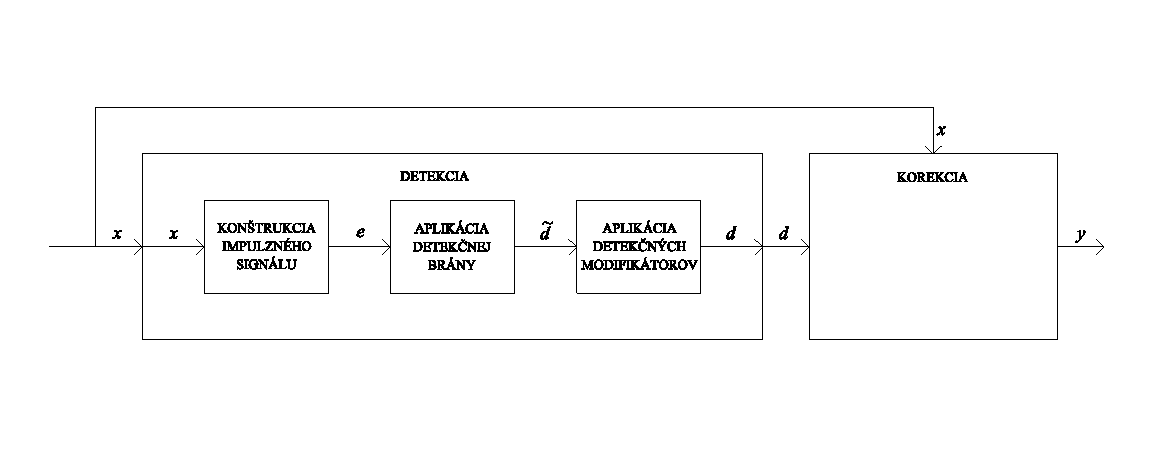
\includegraphics[width=1.0\textwidth]{images/obecny.eps}
	\caption{Schéma obecného algoritmu}
	\label{obrazok:obecny-algoritmus}
\end{figure}

Prácu vybraných algoritmov si môžeme rozdeliť na nasledovné fázy: 
\begin{itemize}
	\item \textit{detekcia} -- lokalizuje poškodené vzorky vstupného znehodnoteného signálu $x$ v podobe výstupného binárneho detekčného signálu $d$. Detekčný signál $d$ je definovaný nasledovým spôsobom:
	$$d_n = \left\{\begin{array}{l l}
		1 & \quad \text{$x_n$ je označená za poškodenú}\\
		0 & \quad \text{$x_n$ je označená za nepoškodenú.}\\
	\end{array} \right.$$
	
	Túto fázu si môže rozdeliť na ďalšie tri fázy:
	\begin{itemize}
		\item \textit{excitácia} -- zo vstupného poškodeného signálu $x$ skonštruuje odpovedajúci excitačný signál $e$. Excitačný signál $e$ má svojou intenzitou zobrazovať pravdepodobnosť poškodenia jednotlivých vzoriek poškodeného signálu $x$.
		\item \textit{aplikácia detekčnej brány} -- určí poškodenosť vzoriek znehodnoteného signálu $x$ z excitačného signálu $e$. Výsledkom aplikácie detekčnej brány na excitačný signál $e$ je prvotná detekcia v podobe binárneho celočíselného detekčného signálu $\tilde{d}$.
		\item \textit{aplikácia detekčného modifikátoru} (nepovinná fáza) -- upraví prvotnú detekciu $\tilde{d}$ na finálnu detekciu $d$. Cieľom aplikácie detekčného modifikátoru je kompenzácia nedostatkov prvotnej detekcie. Detekčných modifikátorov môže byť postupne na prvotnú detekciu $\tilde{d}$ aplikovaných aj viac.
	\end{itemize}
	\item \textit{korekcia} -- opravuje poškodené vzorky vstupného znehodnoteného signálu $x$ na základe detekčného signálu $d$. Výsledkom korekčnej fázy je výstupný opravený signál $y$.
\end{itemize}

Rozdielnosť vybraných algoritmov tkvie najmä v prístupoch ku excitácii a korekcii signálu. Detekčné brány a modifikátory môžu jednotlivé algoritmy zdielať, z toho dôvodu si ich uvedieme v práci až po predstavení vybraných metód. Pre jednotlivé algoritmy si zatiaľ uvedieme len popstupy pre excitáciu a korekciu signálu. Ku opisu detekčnych brán a modifikátorov sa dostaneme na konci tejto kapitoly. Prejdime teraz k predstaveniu algoritmov.

\section{Naivný algoritmus}
Prvý algoritmus, ktorý si uvedieme, je postavený na jednom z najtradičnejších analógových prístupov k čisteniu nahrávok poškodených lokálnymi znehodnoteniami. Vznikol pre účely reštaurovania nahrávok dochovaných na starších nosičoch. Jeho digitálnu variantu máme možnosť vidieť v niektorých súčasných hi-fi súpravách. Algoritmus stavia na predpoklade, že hľadané lokálne poškodenia majú prevažnú časť spektrálneho zastúpenia vo vyšších frekvenciách narozdiel od pôvodného signálu. Je to vďaka malému frekvenčnému rozsahu starších médií.

\subsection{Excitácia}
Naivný algoritmus získava excitačný signál $e$ zo vstupného poškodeného signálu $x$ vyseparovaním pásma vysokých frekvencií. Algoritmov podobného charakteru existuje mnoho, líšia sa typom použitého hornopriepustného filtru pre tieto účely. Naša metóda využije pri excitácii signálu jednoduchú a známu implementáciu hornopriepustného filtru\footnote{Preložené z anglického high pass filter.} založenú na diskrétnej aproximácií druhej derivácie. Tento filter môžeme nájsť v publikácii \cite{Kasparis} pojednávajúcej o algoritme, ktorý si predstavíme v poradí ako druhý. Motiváciou pre hľadanie druhej derivácie je, že derivácia produkuje vysoký výstup len v momentoch náhlych zmien signálu. Inými slovami povedané, zderivovaním signálu zmenšíme intenzitu v ňom obsiahnutých nižších frekvencií. Predpis pre diskrétnu aproximáciu druhej derivácie signálu a teda aj pre výpočet excitačného signálu je nasledujúci: 
$$e_n = x_{n-1} - 2 \cdot x_n + x_{n+1}.$$
Pre väčšiu dynamickú separáciu vyšších frekvencií vstupného poškodeného signálu je možné aplikovať vyššie uvedenú filtráciu opakovane.

\subsection{Korekcia}
Existuje mnoho naivných prístupov ku korekcii nahrávok obsahujúcich lokálne znehodnotenia. Niektoré metódy aplikujú na poškodené časti signálu dolnopriepustný filter\footnote{Preložené z anglického low pass filter.}, iné nahradia každú znehodnotenú vzorku signálu poslednou predchádzajúcou nepoškodenou\footnote{Metóda ``vzorkuj a podrž'', preložené z anglického ``sample and hold''.}. Náš naivný algoritmus sa ku korekcii bude stavať ako ku interpolačnému problému. Každú postupnosť poškodených vzoriek vstupného signálu nahradí vzorkami patriacimi pomyselnej úsečke, ktorá spája dve nepoškodené vzorky priamo susediace s postupnosťou. Formálne, naivným algoritmom opravený signál $y$ získame zo vstupného poškodeného signálu $x$ nasledovne:
$$y_n = \left\{\begin{array}{l l}
	x_n & \quad d_n=0\\
	(1-\frac{o_n}{g_n+1}) \cdot f_n + (\frac{o_n}{g_n+1}) \cdot r_n & \quad d_n=1\\
\end{array} \right.$$
kde $o$ a $g$ sú pomocné celočíselné signály definované nad detekčným signálom $d$:
$$o_n = \left\{\begin{array}{l l}
	0 & \quad d_n=0\\
	n - \max(\{\text{$i$ | $i\leq n$ a $d_i=0$} \}) & \quad d_n=1\\
\end{array} \right.$$
$$g_n = \left\{\begin{array}{l l}
	0 & \quad d_n=0\\
	\min(\{\text{$j$ | $j \geq n$ a $d_j=0$} \}) - \max(\{\text{$i$ | $i \leq n$ a $d_i=0$} \}) - 1 & \quad d_n=1\\
\end{array} \right.$$
a $f$ respektíve $r$ je signál získaný doprednou respektíve dozadnou korekciou spomenutou metódou nahradenia každej znehodnotenej vzorky signálu poslednou predchádzajúcou nepoškodenou:
$$f_n = x_{\max(\{\text{$p$ | $p \leq n$ a $d_p=0$} \})},$$ 
$$r_n = x_{\min(\{\text{$q$ | $q \geq n$ a $d_q=0$} \})}.$$
Táto interpolačná technika je v súčasnosti veľmi populárna vo voľne šíriteľnom software spolu s metódami, ktoré interpolujú sekvencie poškodených vzoriek pomocou Béziérových kriviek.

\section{Kasparis-Laneov algoritmus}
V roku 1993 bola zverejnená metóda, navrhnutá Takisom Kasparisom a Johnom Laneom \cite{Kasparis}, ktorá si podobne ako predchádzajúci algoritmus kládla za cieľ zbaviť staršie audio záznamy praskania. Tento algoritmus vznikol na báze predpokladu, že ku redukcii lokálnych znehodnotení zvukových nahrávok je možné pristupovať podobne ako ku redukcii šumu v digitálnych obrazoch\footnote{Šum ``soľ a korenie'', preložené z anglického salt and pepper noise.}. Veľmi obľúbená metóda na redukciu šumu v digitálnych obrazoch je aplikácia 2D mediánového filtru. Nahradzuje každý pixel digitálneho obrazu mediánom jeho okolitých pixelov. Aplikácia 2D mediánového filtru má však svoje nežiaduce vedľajšie účinky. Vyhladzuje aj oblasti nepoškodené šumom, čím degraduje kvalitu obrazu. Práve kvôli nežiaducej degradácií autori priamu filtráciu vylúčili a navrhli adaptívnu.

\subsection{Excitácia}
Prvý krok algoritmu, ku získaniu excitačného signálu $e$ zo vstupného poškodeného signálu $x$, je rovnaký ako jediný krok nášho naivného algoritmu. Na vstupný signál $x$ aplikujeme hornopriepustný filter založený na diskrétnej aproximácií druhej derivácie, čím získame signál $z$:
$$z_n = x_{n-1} - 2 \cdot x_n + x_{n+1}.$$
Autori metódy po pozorovaní výsledkov aplikácií filtru zistili, že vyfiltrovaný signál $z$ síce relatívne dôveryhodne vypovedá o umiestnení postupností znehodnotených vzoriek, ale nepremieta dostatočne dĺžku ich trvania. Ako ďalší krok preto navrhli aplikáciu operátoru lokálneho kvadratického priemeru na signál $z$:
$$w_n=\frac{1}{2 \cdot Q+1}\sum_{i=-Q}^Q z_{n+i}^2$$ 
kde $Q$ je celočíselný parameter určujúci veľkosť okolia vzoriek pre výpočet lokálneho kvadratického priemeru. Takto získaný signál $w$ pomenovali impulzný signálom. Pri zostavovaní algoritmu sa aplikácia operátoru lokálneho kvadratického priemeru ukázala ako vhodnejší krok, než aplikácia operátoru lokálneho priemeru absolútnej hodnoty vzoriek. Pre získanie excitačého signálu $e$ potrebujeme impulzný signál $w$ na záver znormalizovať jeho referenčným základom $b$. Referenčný základ impulzného signálu $w$ získame aplikáciou rekurzívneho filtru:
$$b_n=med(b_{n-R}, b_{n-(R-1)}, \cdots, b_{n-1}, w_n, w_{n+1}, \cdots, w_{n+R})$$ 
kde $R$ určuje rozsah okolia vzoriek pre výpočet lokálneho mediánu. Keďže je v danej situácií potrebný výpočetne náročný filter, počítajúci v relatívne veľkom okolí, doporučili autori pre efektívnejší výpočt $b$ najskôr zredukovať vzorkovaciu frekvenciu impulzného singálu $w$ celočíselným koeficientom $K$. Redukciou vzorkovacej frekvencie sa efektívne výpočetné okolie rekurzívneho mediánového filtru rozšíri $K$-násobne a tým pádom môže byť výpočet $b$ realizovaný s relatívne menšími parametrami $R$. Excitačný signál $e$ získame nakoniec zo vzťahu: 
$$e_n = \frac{|w_n - b_n|}{b_n}.$$ 
Výsledný signál $e$ je oproti impulznému profilu $w$ údajne prispôsobivejší voči hlasitostným a frekvenčným zmenám v nahrávkach. Schému opísaného procesu môžeme vidieť na obrázku~\ref{obrazok:kasparis-lane}.

\begin{figure}[!h]
	\centering
	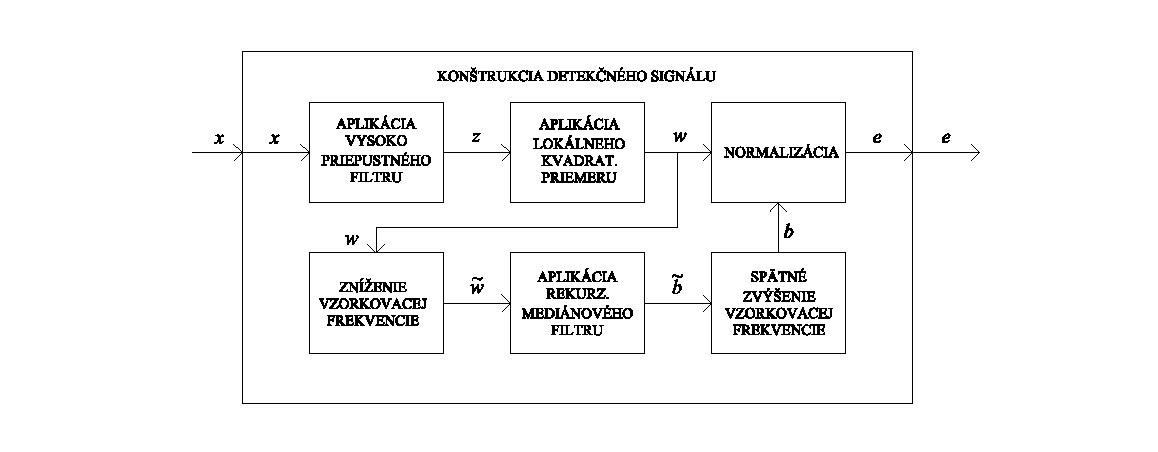
\includegraphics[width=0.8\textwidth]{images/kasparis.eps}
	\caption{Kasparis-Lane: schéma excitácie}
	\label{obrazok:kasparis-lane}
\end{figure}

Pre redukciu vzorkovacej frekvencie signálu $w$ autori algoritmu doporučujú metódu decimácie, ktorú však ďalej nerozvádzajú. V krátkosti si popíšme jednoduchú decimačnú metódu. Potrebné zmenšenie vzorkovacej frekvencie\footnote{Preložené z anglického downsampling.} celočíselným koeficientom $K$ dosiahneme preriedením $l$-vzorkového signálu impulzného profilu $w$ na $\tilde{l}$-vzorkový signál $\tilde{w}$, kde $\tilde{l}=\lceil \frac{l}{K} \rceil$, predpisom: $\tilde{w}_n=w_{n \cdot K}$. Spätné zväčšenie vzorkovacej frekvencie\footnote{Preložené z anglického upsampling.} $\tilde{l}$-vzorkového signálu referenčného základu $\tilde{b}$ (získaného z $\tilde{l}$-vzorkového impuzlného profilu $\tilde{w}$) celočíselným koeficientom $K$ na $m$-vzorkový signál referenčného základu $b$, kde $m=\tilde{l} \cdot K= \lceil \frac{l}{K} \rceil K$, docielime repetizáciou vzoriek: $b_n=\tilde{w}_{\lfloor \frac{n}{K} \rfloor}$.

\subsection{Korekcia}
Pri korekcii autori vylúčili mediánový filter úplne. Myšlienkou bolo aplikovať filter len na znehodnotené vzorky vstupného signálu. Po prevedení sérií experimentov usúdili, že najkvalitnejšie korekčné výsledky sú dosiahnuté aplikáciou mediánového filtru vtedy, keď filter počíta v malých okoliach zahŕňajúcich celé postupnosti poškodených vzoriek. Ako rozumný argument podali fakt, že keď je výpočetné okolie väčšie než postupnosť poškodených vzoriek, sú nové vzorky počítané z väčšej časti signálu a nemodelujú dobre lokálne hodnoty pôvodného signálu. Definitívne riešenie Kasparisa a Lanea pre korekciu poškodených vzoriek je aplikácia adaptívneho mediánového filtru s predpisom: 
$$y_n= med(x_{n-g_n}, \cdots, x_{n+g_n})$$ 
kde $g$ je pomocný celočíselný signál získaný z detekčného signálu $d$ spôsobom popísaným pri naivnom algoritme.


\section{Autoregresívny algoritmus}
V priebehu hľadania efektívnych algoritmov pre detekciu a korekciu lokálnych poškodení digitálnych audio nahrávok sa riešenia začali predovšetkým sústreďovať okolo štatistických prístupov. Štatistické metódy začali nadobúdať experimentálne najlepšie výsledky. Spomedzi pristúpov k signálu ako k časovej rade, je najpopulárnejším autoregresívne modelovanie\footnote{Preložené z anglického autoregressive (AR) modeling.}. Nasledované je kombinovaným autoregresívnym modelovaním s kĺzavými priemermi\footnote{Preložené z anglického autoregressive–moving-average (ARMA) modeling.}. Čisté autoregresívne modely modelujú náhodné procesy, ktorých hodnota v danom čase je váženou sumou konečného počtu bezprostredne predchádzajúcich hodnôt, celkového priemeru časovej rady a náhodnej chybovej zložky. Kombinované autoregresívne modely s kĺzavými priemermi modelujú náhodné procesy, ktorých hodnota v danom čase je váženou sumou konečného počtu bezprostredne predchádzajúcich hodnôt, náhodných chýb konečného počtu bezoprostredne predchádzajúcich predikcií a celkového priemeru časovej rady. Algoritmus, ktorý si uvedieme ako ďalší je založený na autoregresívnom modelovaní. Po jeho predstavení si ukážeme jedno z jeho možných rozšírení. Nasledujúci algoritmus a jeho rozšírenie, ktoré si v práci opíšeme, sú do hĺbky prebraté v publikácii \cite{Godsill} pojednávajúcej o reštaurátorských metódach založených na štatistických prístupoch.

Pri autoregresívnom modelovaní považujeme audio signál za produkt lineárneho časovo-invariantného filtru s nekonečnou impulzívnou odozvou\footnote{Preložené z anglického infinite impulse response (IIR) filter.} aplikovaného na proces Gaussovského bieleho šumu. Formálne vyjadrené:
$$x_n = \sum_{i=1}^P a_i \cdot x_{n-i}+e_n$$ 
kde $x$ je výstupný signál, $P$ je rád autoregresívneho modelu, $a_1$ až $a_P$ sú jeho parametre a $e$ sú vzorky excitačného procesu Gaussovského bieleho šumu. Voľba autoregresívneho modelu je motivovaná faktom, že náhodný excitačný zdroj spolu s modelovým filtrom zdieľa mnohé vlastnosti s reálnymi zvukovými zdrojmi. Napríklad na zvuky ľudksého hlasu môžeme hľadieť ako na náhodné akustické excitácie tvarované fyzickými vlastnosťami majiteľa. Autoregresívny model sme pred kombinovaným autoregresívnym modelom s kĺzavými priemermi uprednostnili kvôli jeho výpočetnej jednoduchosti. Faktom však zostáva, že autoregresívne modelovanie s vyššími rádmi sa správaním dostatočne dobre približuje modelovaniu kombinovaného autoregresívneho modelu s kĺzavými priemermi. 

Algoritmus, ktorý si teraz popíšeme bude pracovať po blokoch digitálnych vzoriek vstupného signálu o veľkosti $B$. Argumentom pre blokové spracovávanie signálu je menšia časová a pamäťová zložitosť výpočtov. Jednotlivé bloky majú tiež jednotnejšie správanie čo sa týka hlasitosti signálu a zastúpenia jednotlivých jeho frekvencií. Pri excitácii respektíve korekcii signálu metóda postupne vytíči blok o veľkosti $B$, poprípade kratší (záleží od počtu zvyšných vzoriek) a následne ho spracuje vo výsledný vektor excitačného respektíve opraveného signálu. Vektory pre jednotlivé bloky priebežne spája v zachovanom poradí vo výsledné signály. Opíšeme si metódu excitácie a korekcie pre daný blok vzoriek.

\subsection{Excitácia}
Majme vstupný poškodený signál $x$, prvý index $i$ a posledný index $j$ pre daný blok. Po obdržaní bloku vzoriek algoritmus najskôr určí odhad parametrov nášho autoregresívneho modelu. Majme teda vektor vstupného poškodeného signálu pre daný blok v tvare:
$$\mathbf{x}=\begin{bmatrix} 
  x_i & x_{i+1} & \cdots & x_j\\ 
\end{bmatrix}^T.$$ 
Chceme odhadnúť vektor parametrov nášho autoregresivneho modelu pre daný blok:
$$\mathbf{a}=\begin{bmatrix} 
  a_1 & a_2 & \cdots & a_P\\
\end{bmatrix}^T.$$ 
Pre odhad parametrov $\mathbf{a}$ daného bloku využijeme metódu najmenších štvorcov. Zostavme si preto autoregresívnu maticu pre daný blok:
$$\mathbf{G}_{AR}=\begin{bmatrix} 
  x_{i-1} & x_{i-2} & \cdots & x_{i-P}\\
  x_i & x_{i-1} & \cdots & x_{i-P+1}\\
  \vdots & \vdots & \ddots & \vdots\\
  x_{j-1} & x_{j-2} & \cdots & x_{j-P}\\
\end{bmatrix}.$$ 
Našim cieľom je určenie parametrov $\mathbf{a}$ vo vzťahu: 
$$\mathbf{x}=\mathbf{G}_{AR} \cdot \mathbf{a} + \mathbf{e}$$ 
kde $\mathbf{e}$ je vektor excitačného signálu pre daný blok v tvare:
$$\mathbf{e}=\begin{bmatrix} 
  e_i & e_{i+1} & \cdots & e_{j}\\
\end{bmatrix}^T.$$
Odhad parametrov autoregresívneho modelu $\mathbf{a}$ získame minimalizáciou vektoru excitačného signálu $\mathbf{e}$: 
$$\mathbf{a}=(\mathbf{G}_{AR}^T \cdot \mathbf{G}_{AR})^{-1} \cdot \mathbf{G}_{AR}^T \cdot \mathbf{x}.$$ 
Takto vytvorený odhad parametrov $\mathbf{a}$ nieje veľmi robustný (robustnejším odhadom je napríklad metóda vážených najmenších štvorcov\footnote{preložené z anglického wighted least squares.}), ale v rámci našej práce si s ním vystačíme. Podstaté je však vedieť, že s robustnejším odhadom parametrov je možné algoritmus zefektívniť. S odhadnutými parametrami $\mathbf{a}$ získame vektor excitačného signálu $\mathbf{e}$ zo vzťahu:
$$\mathbf{e}= \mathbf{x} - \mathbf{G}_{AR} \cdot \mathbf{a}.$$
Vyššie uvedený vzťah predstavuje filtráciu vstupného signálu $x$ pre daný blok filtron autoregresívneho modelu:
$$e_n = x_n - \sum_{i=1}^P a_i \cdot x_{n-i}.$$

\subsection{Korekcia}
Majme vstupný poškodený signál $x$, detekčný signál $d$, prvý index $i$ a posledný index $j$ pre daný blok, na ktorom má prebehnúť korekcia. Ďalej majme signál $y$ obsahujúci opravené vzorky predcházdajúce danému bloku, získané z predošlých výpočtov. Prvý krok ku korekcii do veľkej miery kopíruje začiatok postupu excitácie signálu pre daný blok. Jedná sa o odhadovanie parametrov autoregresívneho modelu, ktoré pri excitácii signálu nemá k dispozicií informáciu o poškodenosti jednotlivých vzoriek. Pri korekcii však už máme k dispozícii detekčný signál $d$. Mnohé algoritmy založené na autoregresívnom modelovaní vytvárajú odhad parametrov pre blok len počas detekcie poškodených vzoriek. S týmito parametrami operujú aj pri korekcii vzoriek v bloku. Ako vlastný návrh si pri korekcii predstavíme metódu opätovného odhadu parametrov autoregresívneho modelu: $$\mathbf{\tilde{a}}=\begin{bmatrix} 
  \tilde{a}_1 & \tilde{a}_2 & \cdots & \tilde{a}_P\\
\end{bmatrix}^T.$$

Pre opätovný odhad parametrov je potrebné najskôr zostaviť autoregresívnu maticu $\mathbf{\tilde{G}}_{AR}$. Maticu $\mathbf{\tilde{G}}_{AR}$ zíkame z matice $\mathbf{G}_{AR}$ (z fázy excitácie signálu pre daný blok) ponechaním len $k$-teho riadku matice pre všetky $k$ také, že $k$-tá vzorka bloku a jej $P$ bezprostredne predchádzajúcich sú v detekcii $d$ označené za nepoškodené. K matici $\mathbf{\tilde{G}}_{AR}$ je potrebný pre opätovný odhad ešte odpovedajúci vektor vstupného signálu $\mathbf{\tilde{x}}$. Ten získame obdobne z vektoru $\mathbf{x}$ (taktiež z fázy excitácie signálu pre daný blok) ponechaním len $k$-teho prvku vektoru pre všetky vyššie uvedené $k$. Opätovný odhad parametrov získame rovnako metódou najmenších štvorcov:
$$\mathbf{\tilde{a}}=(\mathbf{\tilde{G}}_{AR}^T \cdot \mathbf{\tilde{G}}_{AR})^{-1} \cdot \mathbf{\tilde{G}}_{AR}^T \cdot \mathbf{\tilde{x}}.$$ 

Po prevedení opätovného odhadu parametrov $\mathbf{\tilde{a}}$ algoritmus prejde do druhej časti, v ktorej realizuje autoregresívnu interpoláciu metódou najmenších štvorcov\footnote{Preložené z anglického least squares autoregressive (LSAR) interpolation.}. Pre interpoláciu je potrebná matica $\mathbf{A}$ pozostávajúca z novoodhadnutých parametrov $\mathbf{\tilde{a}}$ s počtom riadkov rovným počtu prvkov bloku:
$$\mathbf{A}=\begin{bmatrix}
  -\tilde{a}_P & -\tilde{a}_{P-1} & \cdots & -\tilde{a}_1 & 1 & 0 & \cdots & 0 & 0\\
  0 & -\tilde{a}_P & \cdots & -\tilde{a}_2 & -\tilde{a}_1 & 1 & \cdots & 0 & 0\\
  \vdots & \vdots & \ddots &   \vdots & \vdots & \vdots & \ddots & \vdots & \vdots\\
  0 & 0 & \cdots & 0 & -\tilde{a}_P & -\tilde{a}_{P-1} & \cdots & 1 & 0\\
  0 & 0 & \cdots & 0 & 0 & -\tilde{a}_P & \cdots & -\tilde{a}_1 & 1\\
\end{bmatrix}.$$
Rozdelíme stĺpce matice $\mathbf{A}$ medzi matice $\mathbf{A}_{K}$ a $\mathbf{A}_{U}$ tak, že $k$-ty stĺpec matice bude patriť $\mathbf{A}_{K}$ ak $k \leq P$ alebo je $k$-ta vzorka bloku v $d$ označená za nepoškodenú, inak bude patriť $\mathbf{A}_{U}$. Ďalej je potrebný vektor $\mathbf{y}_{K}$, ktorého prvých $P$ prvkov postupne tvoria vzorky $y_{i-P}$ až $y_{i-1}$ a jeho zvyšné prvky tvoria vzorky bloku signálu $x$, ktoré sú v $d$ označené za nepoškodené (v zachovanom poradí).

Interpolované vzorky nakoniec získame zo vzťahu:
$$\mathbf{y}_{U}=(\mathbf{A}_{U}^{T} \cdot \mathbf{A}_{U})^{-1} \cdot \mathbf{A}_{U}^{T} \cdot \mathbf{A}_{K} \cdot \mathbf{y}_{K}$$ 
kde vektor $\mathbf{y}_{U}$ obsahuje hodnoty opravených vzoriek len pre poškodené vzorky bloku (v zachovanom poradí).

Väčšina algoritmov fungujúcich na podobnom princípe pracuje výhradne len so vzorkami bloku. Takýmto algoritmom sa pri blokovom spracovaní signálu bloky prekrývajú. Nami uvedený algoritmus počíta s $P$ bezprostredne predchádzajúcimi vzorkami pred daným blokom, ktoré už boli algoritmom v predchádzajúch výpočtoch opravené. Táto varianta sa subjektívne osvedčila menej komplikovanou implementáciou. Nasledujúca časť práce bude pojednávať o jednom z možných rozšírení tohto algoritmu.


\section{Sínusoidovo rozšírený autoregresívny algoritmus}
Sínusoidové rozšírenie autoregresívneho algoritmu je založené na princípe podobnom inverznej Fourierovej transformácii\footnote{Preložené z anglického inverse Fourier transform (IFT).}. O jeho teoretických základoch a praktických výsledkoch pojednáva množstvo literatúry, ako napríklad \cite{Godsill}, \cite{Alvarez}. Rozšírený algoritmus predpokladá, že modelovaný signál je možné najskôr do značnej miery vymodelovať sínusoidovým modelom. Ku rozdielovému signálu sa následne správa ako nerozšírený autoregresívny algoritmus. Kombinovaný model rožíreného algoritmu je možné popísať nasledujúcim vzťahom:
$$x_n = \sum_{i=1}^{2 \cdot Q  + 1}c_i \cdot \psi_i[n] + r_n$$
kde $Q$ je rád sinusoidového modelu, $2 \cdot Q +1$ je kardinalita bázy sinusoíd, $\psi_i[n]$ je $n$-tý prvok $i$-tej sínusoidy bázy $\Psi = \left\{ \psi_1, \psi_2, \cdots, \psi_{2 \cdot Q  + 1} \right\}$, jednotlivé váhy lineárnej kombinácie bázy $c_1$ až $c_{2 \cdot Q  + 1}$ sú parametrami sínusového modelu a $r_n$ je zvyšný reziduálny signál, ktorý budeme modelovať autoregresívne: 
$$r_n = \sum_{i=1}^P a_i \cdot r_{n-i}+e_n.$$
Vo vyššie uvedenom vzťahu je $P$ rád autoregresívneho modelu s parametrami $a_1$ až $a_P$ a $e$ sú vzorky excitačného procesu Gaussovského bieleho šumu. 

Rozšírený algoritmus pracuje po blokoch vzoriek veľkosti $B$ rovnako ako jeho nerozšírená varianta. Argument pre blokové spracovávanie zostáva rovnaký.

\subsection{Excitácia}
Majme vstupný poškodený signál $x$, prvý index $i$ a posledný index $j$ pre daný blok. Cieľom algoritmu je získať vektor excitačného signálu pre blok:
$$\mathbf{e}=\begin{bmatrix} 
  e_i & e_{i+1} & \cdots & e_{j}\\
\end{bmatrix}^T.$$ 
Pre výpočet vektoru excitačného signálu najskôr potrebujeme získať vektor reziduálneho signálu pre blok rozširený o $P$ bezprostredne predchádzajúcich vzoriek (kvôli požiadavkám nerozšíreného algoritmu pre výpočet nad daným blokom): 
$$\mathbf{r} =\begin{bmatrix} 
  r_{i-P} & r_{i-P+1} & \cdots & r_{j}\\ 
\end{bmatrix}^T.$$
Z vektoru reziduálneho signálu $\mathbf{r}$ získame vektor excitačného signálu $\mathbf{e}$ metódou rozobranou v časti o nerozšírenom autoregresívnom algoritme. Popíšeme si samotnú konštrukciu vektoru reziduálneho signálu $\mathbf{r}$. 

Pre získanie vektoru reziduálneho signálu je treba najskôr určiť prvky bázy sínusoíd $\Psi$ a následne nato je potrebné vykonať odhad parametrov sínusoidového modelu:
$$\mathbf{c}=\begin{bmatrix} 
  c_1 & c_2 & \cdots & c_{2 \cdot Q  + 1}\\
\end{bmatrix}^T.$$ 

Jeden z možných spôsobov ako zostaviť bázu, je vybrať do $\Psi$ jednosmernú zložku signálu\footnote{Preložené z anglického DC bias.} a $Q$ párov sínusoíd: 
$$\psi_{2 \cdot i - 1}[n]=cos(\omega_i \cdot n \cdot T),$$ 
$$\psi_{2 \cdot i}[n]=sin(\omega_i \cdot n \cdot T)$$
kde $\omega_i$ je frekvencia $i$-tej sínusoidy a $T$ je vzorkovací interval digitálneho signálu. Pri implementácií sa nám osvedčil iný adaptívnejší prístup k zostaveniu bázy, ktorý počíta s charakterom signálu v danom bloku. Do $\Psi$ najskôr zaradíme jednosmernú zložku signálu. Zvyšné sínusoidy zvolíme podľa výsledkov aplikácie diskrétnej Fourierovej transformácie\footnote{Preložené z anglického discrete Fourier transform (DFT).} na vektor vstupného poškodeného signálu pre blok rozšírený o $P$ bezprostredne predchádzajúcich vzoriek danému bloku: 
$$\mathbf{x} =\begin{bmatrix} 
  x_{i-P} & x_{i-P+1} & \cdots & x_{j}\\
\end{bmatrix}^T.$$
Z výsledku aplikácie diskrétnej Fourierovej transformácie na vektor $\mathbf{x}$ vyberieme do sínusoidovej bázy $Q$ párov funkcií sínus a kosínus, odpovedajúcich najzástupenejším frekvenciám v bloku, prvým popísaným spôsobom. Ku zostavenej báze $\Psi$ potrebujeme určiť váhy prvkov v podobe parametrov sínusoidového modelu $\mathbf{c}$. Pre odhad parametrov $\mathbf{c}$ metódou najmenších štvorcov je potrebná matica:
$$\mathbf{G}_{SIN} =\begin{bmatrix} 
  \psi_{1}[1] & \psi_{2}[1] & \cdots & \psi_{2 \cdot Q  + 1}[1]\\
  \psi_{1}[2] & \psi_{2}[2] & \cdots & \psi_{2 \cdot Q  + 1}[2]\\
  \vdots & \vdots & \ddots & \vdots\\
  \psi_{1}[n] & \psi_{2}[n] & \cdots & \psi_{2 \cdot Q  + 1}[n]\\
\end{bmatrix}$$
kde $n$ je počet prvkov vektoru $\mathbf{x}$. S maticou $\mathbf{G}_{SIN}$ a vektorom poškodeného signálu $\mathbf{x}$ získame odhad parametrov $\mathbf{c}$ zo vzťahu:
$$\mathbf{c}=(\mathbf{G}_{SIN}^{T} \cdot \mathbf{G}_{SIN})^{-1} \cdot \mathbf{G}_{SIN}^T \cdot \mathbf{x}.$$ 

Vektor reziduálneho signálu $\mathbf{r}$ pre blok nakoniec dostaneme vyjadrením:
$$\mathbf{r} = \mathbf{x} - \mathbf{G}_{SIN} \cdot \mathbf{c}.$$

\subsection{Korekcia}
Majme vstupný poškodený signál $x$, detekčný signál $d$, prvý index $i$ a posledný index $j$ pre daný blok určený na korekciu. Ďalej majme signál $y$ obsahujúci opravené vzorky predchádzajúce danému bloku, získané z predošlých výpočtov. Sínusoidovú bázu $\tilde{\Psi}$ pre blok zostavíme metódou popísanou pri excitácii aplikovanou na vektor vstupného signálu rozšíreného o $P$ predom opravených bezprostredne predchádzajúcich vzoriek danému bloku:
$$\mathbf{\tilde{x}} =\begin{bmatrix} 
  y_{i-P} & y_{i-P+1} & \cdots & y_{i-1} & x_{i} & x_{i+1} &\cdots & x_{j}\\
\end{bmatrix}^T.$$
S určenou bázou $\tilde{\Psi}$ odhadneme z vektoru $\mathbf{\tilde{x}}$ parametre sínusoidového modelu $\mathbf{\tilde{c}}$ spôsobom popísaným pri excitácii. Vektor reziduálneho signálu získame následne zo vzťahu:
$$\mathbf{\tilde{r}} = \mathbf{\tilde{x}} - \mathbf{\tilde{G}}_{SIN} \cdot \mathbf{\tilde{c}}.$$
kde maticu $\mathbf{\tilde{G}}_{SIN}$ zostavíme metódou popísanou pri excitácii z bázy $\tilde{\Psi}$. 

Na reziduálny signál v podobe vektoru $\mathbf{\tilde{r}}$ s detekčným signálom $d$ aplikujeme korekciu nerozšíreného algoritmu pre blok začínajúci na $P$-tej vzorke a končiaci na konci vektoru $\mathbf{\tilde{r}}$. Získame opravený reziduálny signál pre blok $\mathbf{\tilde{y}}$. 

Výsledný vektor opraveného signálu pre blok vznikne sčítaním vektoru signálu modelovaného sínusoidovým modelom pre daný blok s vektorom opraveného reziduálneho signálu $\mathbf{\tilde{y}}$.

\section{Algoritmus založený na neurónovej sieti}
Algoritmus, ktorý sa chystáme predstaviť, je vlastnou aplikáciou umelých neurónových sietí na danú problematiku. Umelá neurónová sieť je výpočtový model, ktorý vznikol na základe abstrakcie z biologických neurónových systémov. Základnou stavebnou jednotkou neurónovej siete je neurón, pre ktorý existuje niekoľko modelov. V našej neurónovej sieti využijeme jeden z najpoužívanejších model neurónu, ktorý zavedený McCullochom a Pittsom. Môžeme ho popísať nasledovným vzťahom:
$$b = S(\sum_{i=1}^{N}(w_i \cdot a_i) + \Theta)$$
kde $a_i$ sú vstupy neurónu, $w_i$ sú synaptické váhy, $\Theta$ je prah, $S(a)$ je aktivačná funckia a $b$ je výstup neurónu.
Jednotlivé neuróny sú vzájomne poprepájané do siete. Model siete ktorý využijeme v našom algoritme je známy pod menom viacvrstvový perceptrón\footnote{Preložené z anglického Multilayer perceptron} a patrí medzi dopredné vrstevnaté siete. V takýchto sietiach sú neuróny usporiadané do vrstiev a synapsie spájajú všetky dvojice neurónov susedných vrstiev. Konkrétny príklad viacvrstvového perceptrónu môžeme vidieť na obrázku~\ref{obrazok:neuronova-siet}.

\begin{figure}[!h]
	\centering
	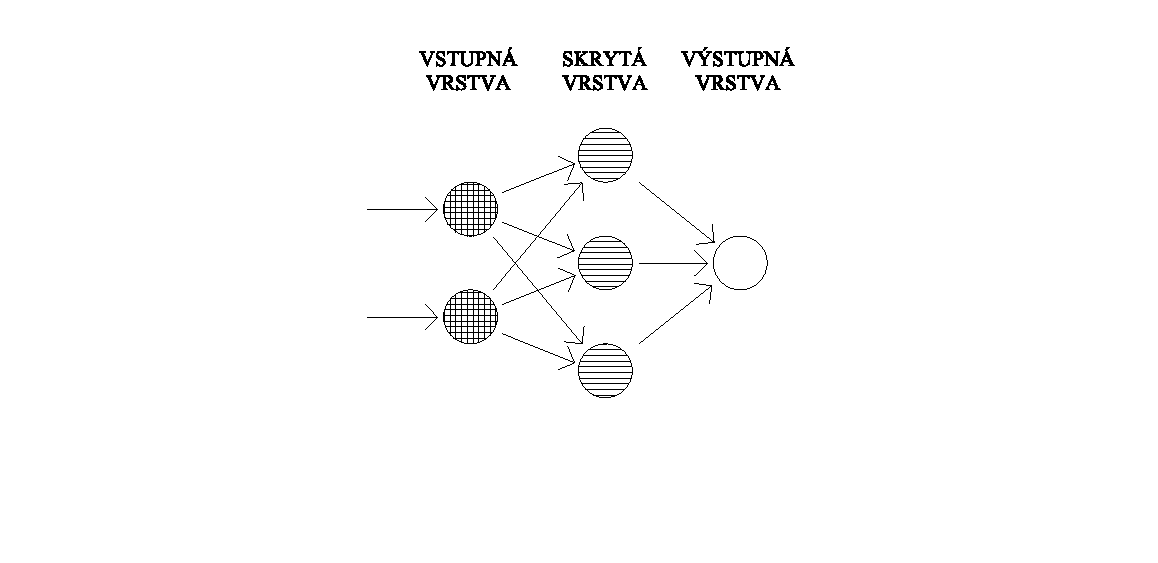
\includegraphics[width=1.0\textwidth]{images/siet.eps}
	\caption{Viacvrstvový perceptrón}
	\label{obrazok:neuronova-siet}
\end{figure}

V práci použijeme algoritmus učenia s učiteľom pomocou spätného šírenia chyby, čo je najpoužívanejší algoritmus učenia tohto druhu sietí. Viacvrstvový perceptrón realizuje nelineárnu funkciu z množiny možných vstupov do množiny príslušných výstupov. Už sme si predstavili algoritmus založený na lineárnom autoregresívnom modeli. Viacvrstvový perceptrón je rozšírením myšlienky lineárneho perceptrónu, ktorého možnosti sú teoreticky rovnaké ako možnosti autoregresívneho modelu. Motiváciou implementácie tohto algoritmu je otázka nakoľko si pri riešení nášho problému polepšíme prechodom z lineárneho na nelineárny model. Spoľahlivým zdrojom ďalších informácií o neurónových sietiach je \cite{Sima}. 

Podobne ako algoritmus založený na autoregresívnom modeli, bude aj tento pracovať po blokoch digitálnych vzoriek zo vstupného signálu o veľkosti $B$. Dôvodom pre blokové spracovávanie signálu naďalej zostáva menšia časová a pamäťová zložitosť výpočtu a jednotnejší hlasitostný aj frekvenčný charakter. Pre rámec algoritmu prepokladajme, že máme k dipozícii viacvrstvový perceptrón s počtom vstupných neurónov $N$, jedným výstupným neurónom a $H$ neurónmi v skrytej vrstve. Tréningy budú prebiehať v $T$-cyklovej iterácii s učiacim koeficientom $L$.

\subsection{Excitácia}
Majme daný vstupný poškodený signál $x$, prvý index $i$ a posledný index $j$ pre daný blok. Metóda si v prvom rade zostaví tréningovú množinu pre sieť zo vzoriek bloku. Táto tréningová množina pozostáva z dvojíc vstupného vektoru dĺžky $N$ a výstupného vektoru dĺžky $1$. Pre každú vzorku daného bloku zaradíme do tréningovej množiny dvojicu vstupného vektoru obsahujúceho $N$ bezprostredne predchádzajúcich vzoriek danej vzorke (v zachovanom poradí) a výstupného vektoru obsahujúceho len danú vzorku. Inými slovami, pre všetky indexy $k$ daného bloku zaradíme do tréningovej množiny dvojicu vstupného vektoru $\mathbf{a}_k$ a výstupného vektoru $\mathbf{b}_k$:
$$\mathbf{a}_k=\begin{bmatrix} 
x_{k-N} & x_{k-N+1} & \cdots & x_{k-1}\\
\end{bmatrix}^T,$$
$$\mathbf{b}_k=\begin{bmatrix} 
x_k\\ 
\end{bmatrix}^T.$$
Takto zostavenou tréningovou množinou natrénujeme našu sieť algoritmom učenia s učiteľom pomocou spätného šírenia chyby. 

Za pomoci natrénovanej získame vektor excitačného signálu pre daný blok:
$$\mathbf{e}=\begin{bmatrix} 
  e_i & e_{i+1} & \cdots & e_{j}\\
\end{bmatrix}^T$$ 
tak, že jednotlivé excitácie $e_k$ vyjadríme odčítaním predikovanej vzorky od poškodenej:
$$e_k = x_k - p_k.$$ 
V uvedenom vzťahu je predikovaná vzorka $p_k$ rovná jedinému prvku výstupného vektoru natrénovanej siete pre vstupný vektor $\mathbf{a}_k$.

\subsection{Korekcia}
Pri oprave poškodeného signálu algoritmus najskôr vykoná doprednú korekciu vstupného signálu $x$ s detekčným signálom $d$, po ktorej obdrží signál $f$. Ďalej vykoná druhú doprednú korekciu nad obrátenými signálmi $x$ a $d$, z ktorej opravený signál opätovne obráti vo výsledný opravený signál $r$. Proces získania signálu $r$ nazveme spätnou korekciou. Dopredná aj spätná korekcia prebieha postupne po blokoch poškodeného signálu o veľkosti $B$. Po tom, čo algoritmus získa dopredný aj spätný opravený signál vyhotoví finálnu korekciu v podobe signálu $y$. Princíp výpočtu finálnej korekcie z doprednej a spätnej si vysvetlíme na záver. Opíšme si najskôr metódu doprednej korekcie pre daný blok.

Majme vstupný poškodený signál $x$, jemu odpovedajúci detekčný signál $d$, prvý index $i$ a posledný index $j$ pre daný blok, na ktorom má prebehnúť dopredná korekcia. Ďalej majme signál $y$ obsahujúci dopredne opravené vzorky predchádzajúce danému bloku, získané z predošlých výpočtov. Metóda zostaví tréningovú množinu, do ktorej zaradí pre každú vzorku daného bloku, ktorá je spolu s jej $N$ bezprostredne predchadzajúcimi vzorkami v detekcii $d$ označená za nepoškodenú, dvojicu vstupného vektoru obsahujúceho $N$ bezprostredne predchádzajúcich vzoriek danej vzorke (v zachovanom poradí) a výstupného vektoru obsahujúceho len danú vzorku. Inými slovami, pre všetky indexy $k$ daného bloku, pre ktoré $k$-ta vzorka vstupného signálu spolu s jej $N$ bezprostredne predchádzajúcimi vzorkami sú v detekčnom signáli $d$ označené za nepoškodené, zahrnieme do tréningovej množiny dvojicu vstupného vektoru $\mathbf{a}_k$ a výstupného vektoru $\mathbf{b}_k$:
$$\mathbf{a}_k=\begin{bmatrix} 
x_{k-N} & x_{k-N+1} & \cdots & x_{k-1}\\ 
\end{bmatrix}^T,$$
$$\mathbf{b}_k=\begin{bmatrix} 
x_k\\ 
\end{bmatrix}^T.$$
Pripravenou tréningovou množinou natrénujeme našu sieť metódou učenia s učiteľom pomocou spätného šírenia chyby. 

V ďalšej časti algoritmu natrénovaná sieť poskytuje predikcie pre jednotlivé poškodené vzorky. Pri implementácii sa osvedčil dopredný prechod v rámci bloku s nahradením každej poškodenej vzorky predikovanou. Pri výpočte predikcie metóda počíta s predom vykonanými predikciami namiesto toho aby brala do úvahy poškodené vzorky. Výsledný dopredne opravený vektor získame vyjadrením:
$$\mathbf{f}=\begin{bmatrix} 
  f_i & f_{i+1} & \cdots & f_{j}\\
\end{bmatrix}^T$$ 
kde jednotlivé $f_k$ získame rekurzívne zo vzťahu:
$$f_k = \left\{\begin{array}{l l}
	y_k & \quad \text{$k<i$}\\
	x_k & \quad \text{$k\geq i$ a $d_k=0$}\\
	p_k & \quad \text{inak}\\
\end{array} \right.$$
kde predikcia $p_k$ je rovná jedinému prvku výstupného vektoru natrénovanej siete pre vstupný vektor:
$$\mathbf{f}_k=\begin{bmatrix} 
f_{k-N} & f_{k-N+1} & \cdots & f_{k-1}\\ 
\end{bmatrix}^T.$$

Konečný opravený signál $y$ získame zložením signálov doprednej $f$ a spätnej korekcie $r$ zo vzťahu:
$$y_n = \left\{\begin{array}{l l}
	x_n & \quad d_n = 0\\
	(1-\frac{o_n}{g_n+1}) \cdot f_n + (\frac{o_n}{g_n+1}) \cdot r_n & \quad d_n=1.\\
\end{array} \right.$$
Celočíselné pomocné signály $g$ a $o$ získame z detekčného signálu $d$ spôsobom popísaným v časti o naivnom algoritme.

\section{Detekčné brány}
V časti práci pojednávajúcej o obecnom algoritme pre reštaurovanie nahrávok poškodených lokálnymi znehodnoteniami bolo uvedené, že v druhej fáze detekcie sa na excitačný signál $e$ aplikuje detekčná brána. Úlohou detekčnej brány je určiť prvotnú detekciu poškodených vzoriek signálu $x$ v podobe binárneho detekčného signálu $\tilde{d}$. Popíšeme si princípy niekoľkých detekčných brán.

\subsection{Jednoduchá detekčná brána}
Jednoduchá detekčná brána v detekcii $\tilde{d}$ označí za poškodené tie vzorky, ktorých absolútna hodnota excitácie je väčšia než stanovený prah $T$. Detekciu získanú aplikáciou jednoduchej detekčnej brány na excitačný signál $e$ je možné formálne vyjadriť predpisom:
$$\tilde{d}_n = \left\{\begin{array}{l l}
	1 & \quad  |e_n|>T\\
	0 & \quad \text{inak}\\
\end{array} \right.$$
kde $T$ je prah brány. Veľkým nedostatkom jednoduchej detekčnej brány je absolútna neadaptívnosť voči charakteru excitačných signálov. Pre naše účely je jednoduchá detekčná brána takmer nepoužiteľná. V práci je predstavená len pre počiatočnú ilustráciu princípu fungovania brán.

\subsection{Detekčná brána smerodajnej odchýlky}
Nasledujúca brána je prispôsobivejšia než predchádzajúca jednoduchá. Detekčná brána smerodajnej odchýlky čiastočne prihliada pri detekcií poškodených vzoriek na charakter intenzity excitačného signálu. Detekčný signál $\tilde{d}$ získaný aplikáciou brány smerodajnej odchýlky na excitačný signál $e$ môžeme vyjadriť vzťahom:
$$\tilde{d}_n = \left\{\begin{array}{l l}
	1 & \quad |e_n|> P \cdot \sigma\\
	0 & \quad \text{inak.}\\
\end{array} \right.$$
kde $P$ je prahový parameter brány a $\sigma$ je smerodajná odchýlka excitačného signálu $e$. Jedným zo spôsobov ako získať smerodajú odchýlku $\sigma$ je priamym výpočtom zo známeho vzťahu:
$$\sigma=\sqrt{\frac{1}{N} \cdot \sum_{i=1}^N(e_i-\bar{e})^2}$$
kde $\bar{e}$ je priemerná hodnota vzorky excitačného signálu:
$$\bar{e}=\frac{1}{N} \cdot \sum_{i=1}^N(x_i).$$

Smerodajnú odchýlku $\sigma$ excitácií môžeme taktiež získať pomocou metódy robustnej aproximácie, ktorá bola zavedená Kleinerom a Martinom v ich práci \cite{Kleiner}. Kleiner-Martinova aproximačná metóda je v praxi bežne používana pre podobné účely. Jej predpis je nasledovný:
$$\sigma \approx \frac{med(|e|)}{0,6745}$$
kde $med(|e|)$ je medián absolútnych hodnôt vzoriek excitačného signálu $e$.
Detekčná brána smerodajnej odchýlky je vhodnou voľbou v situáciách, kedy nemá excitačný signál vo svojom priebehu premenlivú intenzitu.

\subsection{Adaptívna detekčná brána smerodajnej odchýlky}
Existuje mnoho spôsobov, akými by sme mohli získať bránu adaptívnu voči premenlivej intenzite excitácií. Jedno z možných riešení je nechať predošlú bránu počítať detekciu po blokoch vzoriek excitačného signálu. V takomto prípade by boli štandardné odchýlky a nimi určené prahy počítané lokálne zvlášť pre každý blok. Predstavme si vlastnú prispôsobivú bránu smerodajnej odchýlky, ktorá počíta detekciu vzhľadom na vzorkové okolie. Detekčný signál $\tilde{d}$ adaptívnej detekčnej brány smerodajnej odchýlky získame z excitačného signálu $e$ predpisom:
$$\tilde{d}_n = \left\{\begin{array}{l l}
	1 & \quad |e_n|> P \cdot \sigma_n\\
	0 & \quad \text{inak}\\
\end{array} \right.$$
kde $P$ je prahový parameter brány a $\sigma_n$ je lokálna smerodajná odchýlka excitácií:
$$\sigma_n=\sqrt{\frac{1}{2 \cdot R+1}\sum_{i=-R}^{R}(e_{n+C \cdot i} - \bar{e}_n})^2.$$
Vo vyššie uvedenom vzťahu je $R$ respektíve $C$ celočíselný koeficient vyjadrujúci rozsah respektíve decimáciu vzorkového okolia lokálneho výpočtu a $\bar{e}_n$ je lokálny priemer vzoriek excitácií:
$$\bar{e}_n=\frac{1}{2 \cdot R+1} \cdot \sum_{i=-R}^{R}e_{n+C \cdot i}.$$

Pre výpočet lokálnej smerodajnej odchýlky excitácií môžeme opäť použiť zmienenú aproximáčnú metódu navrhnutú Kleinerom a Martinom:
$$\sigma_n \approx \frac{med(|e_{n-C \cdot R}|, |e_{n-C \cdot (R-1)}|\cdots, |e_{n+C \cdot R}|)}{0,6745}.$$ 

Čo sa týka brán, nieje prispôsobivosť vždy žiadúcou vlastnosťou. Vhodnosť aplikácie adaptívnej brány záleží od pravidelnosti rozloženia lokálnych znehodnotení vo vstupnom poškodenom signáli.


\subsection{Systém dvoch prahov}
Systém detekčných brán, ktorého princíp si teraz opíšeme, je celkom univerzálny a je ho možné aplikovať na všetky v práci spomenuté brány. Jeho hlavnou myšlienkou je zaviesť dva prahy pre detekciu poškodených vzoriek z excitačného signálu. Prvý prah slúži k určeniu poškodenosti vzorky na začiatku postupnosti poškodených. Druhý prah slúži k určeniu poškodenosti vzorky uprostred postupnosti poškodených. 

Implementáciu systému do jednoduchej detekčnej brány získame zavedením dvoch prahov $T_1$, $T_2$ namiesto jediného $T$. Výsledný detekčný signál takto upravenej jednoduchej brány môžeme vyjadriť nasledovne:
$$\tilde{d}_n = \left\{\begin{array}{l l}
	1 & \quad \text{$|e_n|>T_1$ a $d_{n-1}=0$ alebo}\\
	 & \quad \text{$|e_n|>T_2$ a $d_{n-1}=1$}\\
	0 & \quad \text{inak}.\\
\end{array} \right.$$

Implementáciu systému do zvyšných z uvedených brán získame napríklad nahradením jediného prahového parametru $P$ dvomi novými $P_1$, $P_2$. 

Princíp dvoch prahov detekčných brán vznikol vďaka charakteru historických analógových médií a vlastnostiam im prislúchajúcich lokálnych znehodnotení. Tieto poškodenia mávajú zvyčajne začiatok intenzivnejší než svoj zvyšok, a to sa premieta aj do mnohých excitačných signálov.


\section{Detekčné modifikátory}
Poslednú nepovinnú fázu detekcie tvoria aplikácie detekčných modifikátorov. Tie pracujú s prvotnou detekciou poskytnutou detekčnou bránou v podobe signálu $\tilde{d}$. Cieľom aplikácií modifikátorov je skvalitnenie prvotných detekcií vo výsledný detekčný signál $d$. V rámci práce si predstavíme tri modifikátory, ktoré pri vhodnom použití redukujú nedostatky prvotných detekcií.

\subsection{Detekčný rozširovač}
Detekčný rozširovač upraví detekciu $\tilde{d}$ vo výslednú $d$ tak, že každú vzorku $\tilde{d}_n$ s danou binárnou hodnotou $L$ duplikuje na $P$ pozícií $dopredu$ alebo $dozadu$ prípadne $obecne$. Výslednú detekciu $d$ môžeme vyjadriť nasledovne:
$$d_n = \left\{\begin{array}{l l}
	L & \quad \text{$dopredu$ a $\exists i : (i \leq n$ a $\tilde{d}_i=L$ a $|n-i| \leq P$) alebo}\\
	& \quad \text{$dozadu$ a $\exists i : (i \geq n$ a $\tilde{d}_i=L$ a $|n-i| \leq P$) alebo}\\	
	& \quad \text{$obecne$ a $\exists i : (\tilde{d}_i=L$ a $|n-i| \leq P$)}\\
	1-L & \quad \text{inak}.\\
\end{array} \right.$$

\subsection{Detekčný prepájač}
Detekčný prepájač upraví detekciu $\tilde{d}$ tak, že každú dvojicu vzoriek $\tilde{d}_i$, $\tilde{d}_j$ s danou binárnou hodnotou $L$, ktorých vzájomná vzdialenosť je menšia ako parameter $P$, prepojí vo výslednom detekčnom signáli $d$ hodnotami $L$ na medzipozciách. Formálne môžeme výslednú detekciu $d$ vyjadriť:
$$d_n = \left\{\begin{array}{l l}
	L & \quad \min(\{\text{$j$ | $j \geq n$ a $\tilde{d}_j=L$} \}) - \max(\{\text{$i$ | $i \leq n$ a $\tilde{d}_i=L$} \}) \leq P\\
	1-L & \quad \text{inak}.\\
\end{array} \right.$$

\subsection{Detekčný posúvač}
Detekčný rozširovač upraví detekciu $\tilde{d}$ vo výslednú $d$ tak, že každú jeho vzorku posunie o $P$ pozícii $dopredu$ alebo $dozadu$. Výslednú detekciu $d$ môžeme vyjadriť nasledovne:
$$d_n = \left\{\begin{array}{l l}
	\tilde{d}_{n-P} & \quad dopredu\\
	\tilde{d}_{n+P} & \quad dozadu.\\
\end{array} \right.$$
%%%%%%%%%%%%%%%%%%%%%%%%%%%%%%%%%%%%%%%%%%%%%%%%%%%%%%%%%%%%%%%%%%%%%%%%%%%%%%%%
%% BAKALÁRSKA PRÁCA                                                           %%
%%                                                                            %%
%% Názov (sk): Algoritmy detekcie a korekcie lokálnych                        %%
%%             znehodnotení digitálneho audio signálu                         %%
%% Názov (en): Algorithms for Detection and Correction of Local               %%
%%             Degradations in Digital Audio Signals                          %%
%%                                                                            %%
%% Autor: Jakub Kúdela                                                        %%
%% Vedúci: Mgr. Daniel Toropila                                               %%
%%                                                                            %%
%% Akademický rok: 2011/2012                                                  %%
%%%%%%%%%%%%%%%%%%%%%%%%%%%%%%%%%%%%%%%%%%%%%%%%%%%%%%%%%%%%%%%%%%%%%%%%%%%%%%%%

\chapter{Knižnica DAPNet}
Pre účely realizácie pozorovania schopností algoritmov popísaných v práci vznikla vlastná knižnica. Napísaná je v objektovo orientovanom programovacom jazyku C\# s názvom DAPNet\footnote{Skrátene z anglického .Net Digital Audio Processing Library.}. Knižnica DAPNet umožňuje svojim uživateľom editáciu digitálnych audio nahrávok uložených v súboroch formátu WAV. Súbor WAV, osem alebo šesnásť bitového charakteru, umožnuje načítať do operačnej pamäti. Vzorky načítaných nahrávok v pamäti je následne možné editovať. Po vykonaní editácie je možné upravenú nahrávku spätne uložiť na pevný disk. V súčasnosti knižnica obsahuje niekoľko offline implementácií digitálnych audio efektov. Medzi ne patria napríklad signálový zosilovač a normalizér, mediánový a vysokopriepustný filter. Knižnica obsahuje aj všetky metódy pre detekciu a korekciu lokálnych znehodnotení signálov predstavených v tejto práci. Kód~\ref{kod} poskytuje ukážku práce s knižnicou DAPNet. Program najskôr načíta poškodenú nahrávku a aplikuje na ňu algoritmus založený na autoregresívnom modeli. Pred tým, než nahrávku uloží do nového súboru, ju ešte znormalizuje.

\lstinputlisting[caption=Ukážka, label=kod]{codes/example.cs}

\section{Architektúra}
Na vyššie uvedenom kóde~\ref{kod} si popíšme najpodstatnejšie triedy knižnice DAPNet. Trieda pomenovaná \texttt{Wave} je reprezentáciou digitálnej audio nahrávky formátu WAV. Metódy \texttt{Wave.Read} a \texttt{Wave.Write} čítajú a ukladajú nahrávky. Trieda \texttt{Wave} má vlastnosť \texttt{Wave.Channels}, ktorá vracia pole kanálových stôp danej nahrávky. Kanálové stopy sú inštanciami triedy \texttt{SampleVector}. Táto trieda predstavuje indexovateľnú kolekciu vzoriek uložených v hodnotovom type \texttt{double}. Na jednotlivé stopy je možné aplikovať audio efekty implementujúce abstraktnú triedu \texttt{Effect} s abstraktnou metódou \texttt{Effect.Process}. Trieda normalizéru \texttt{PeakNormalizer} z ukážky~\ref{kod} je jednoduchým príkladom implementácie triedy \texttt{Effect}. 

V úvode kapitoly už bolo spomenuté, že knižnica DAPNet obsahuje všetky metódy pre odstraňovanie lokálnych znehodnotení z nahrávok. Jednotlivé algoritmy, detekčné brány a modifikátory sú reprezentované postupne abstraktnými triedami \texttt{Declicker}, \texttt{DetectionGate} a \texttt{DetectionModificator}. Binárnemu detekčnému signálu odpovedá trieda \texttt{DetectionVector}. Je to indexovaťelná kolekcia binárnych vzoriek uložených v hodnotovom type \texttt{bool}. Dizajn tried \texttt{Declicker}, \texttt{DetectionGate} a \texttt{DetectionModificator} odpovedá zobecneniu, ktoré sme si uviedli na začiatku práce. Pre realizáciu algoritmu poskytujúceho excitáciu a korekciu poškodeného signálu v zmysle knižce DAPNet, je potrebné implementovať triedu \texttt{Declicker} definovaním metód \texttt{Declicker.GetExcitations} a \texttt{Declicker.Correct}. Metóda \texttt{Declicker.GetExcitations} vracia pre vstupný signál excitačný a metóda \texttt{Declicker.Correct} opravuje signál na základe poskytnutej detekcie. V ukážkovom kóde~\ref{kod} máme možnosť vidieť volanie algoritmu založenom na autoregresívnom modeli. Je reprezentovaný inštanciou triedy \texttt{ARDeclicker}. 

Rozhranie abstraktnej triedy brány \texttt{DetectionGate} si vynucuje implementáciu metódy \texttt{DetectionGate.Detect}. Metóda \texttt{DetectionGate.Detect} vracia pre vstupný signál prvotnú detekciu. Detekčnou bránou vo vyššie uvedenom kóde~\ref{kod} je inštancia triedy \texttt{DeviationSimpleGate}. Predstavuje jednoduchú bránu smerodajnej odchýlky s jedným prahom. 

Modifikátory implementujú metódu \texttt{DetectionModificator.Modify}. Metóda \texttt{DetectionModificator.Modify} pracuje len s binárnym detekčným signálom, ako bolo uvedené pri opise obecného algoritmu. V kóde~\ref{kod} predstavuje detekčný modifikátor inštancia triedy \texttt{DetectionWidener}. Reprezentuje detekčný rozširovač popísaný v práci. 

Nasledujúce zoznamy zoskupené v tabuľkách~\ref{tabulka:algoritmy},~\ref{tabulka:brany} a~\ref{tabulka:modifikatory} sú zhrnutiami tried knižnice DAPNet implementujúcich metódy detekcie a korekcie lokálnych znehodnotení popísaných v práci:

\begin{table}[!h]
\centering
\caption{Algoritmy v DAPNet}
\begin{tabular}{l l}
\hline
Trieda & Algoritmus\\
\hline
\texttt{NDeclicker} & naivný\\
\texttt{KLDeclicker} & Kasparis-Laneov\\
\texttt{ARDeclicker} & autoregresívny\\
\texttt{SARDeclicker} & sínusoidovo rozšírený autoregresívny\\
\texttt{NNDeclicker} & založený na neurónovej sieti\\
\hline
\end{tabular}
\label{tabulka:algoritmy}
\end{table}

\begin{table}[!h]
\centering
\caption{Detekčné brány v DAPNet}
\begin{tabular}{l l}
\hline
Trieda & Detekčná brána\\
\hline
\texttt{SimpleGate} & jednoduchá \\
\texttt{DoubleGate} & jednoduchá s dvomi prahmi\\
\texttt{DeviationSimpleGate} & smerodajnej odchýlky \\
\texttt{DeviationDoubleGate} & smerodajnej odchýlky s dvomi prahmi\\
\texttt{AdaptiveSimpleGate} & adaptívna smerodajnej odchýlky\\
\texttt{AdaptiveDoubleGate} & adaptívna smerodajnej odchýlky s dvomi prahmi\\
\hline
\end{tabular}
\label{tabulka:brany}
\end{table}

\begin{table}[!h]
\centering
\caption{Detekčné modifikátory v DAPNet}
\begin{tabular}{l l}
\hline
Trieda & Detekčný modifikátor\\
\hline
\texttt{DetectionWidener} & rozširovač\\
\texttt{DetectionJoiner} & prepájač\\
\texttt{DetectionShifter} & posúvač\\
\hline
\end{tabular}
\label{tabulka:modifikatory}
\end{table}

\section{Použité knižnice}
V implementácii knižnice DAPNet bolo použitých niekoľko knižníc. V prvom rade je to matematická knižnica MathNet.Numerics \cite{Numerics}. Poskytuje knižnici DAPNet hlavne metódy pre riešenie sústav rovníc a Bluesteinov algoritmus pre výpočet rýchlej Fourierovej transformácie\footnote{Preložené z anglického Bluestein's Fast Fourier Transform algorithm.} nad vektorom arbitrárnej veľkosti. Pri implementácii vlastného návrhu algoritmu založenom na neurónovej sieti bola využitá knižnica NeuronDotNet \cite{NeuronDotNet}, ktorá poskytla výpočetný model viacvrstvového perceptrónu. V poslednom rade bola použitá knižnica ZedGraph \cite{ZedGraph} pre vykreslovanie grafov v okennej aplikácii s názvom DeclickerInspector, ktorú bude predstavená v nasledujúcej kapitole. Dôležité je spomenúť, že pri práci s uvedenými knižnicami nedošlo k porušeniu licenčných podmienok.
%%%%%%%%%%%%%%%%%%%%%%%%%%%%%%%%%%%%%%%%%%%%%%%%%%%%%%%%%%%%%%%%%%%%%%%%%%%%%%%%
%% BAKALÁRSKA PRÁCA                                                           %%
%%                                                                            %%
%% Názov (sk): Algoritmy detekcie a korekcie lokálnych                        %%
%%             znehodnotení digitálneho audio signálu                         %%
%% Názov (en): Algorithms for Detection and Correction of Local               %%
%%             Degradations in Digital Audio Signals                          %%
%%                                                                            %%
%% Autor: Jakub Kúdela                                                        %%
%% Vedúci: Mgr. Daniel Toropila                                               %%
%%                                                                            %%
%% Akademický rok: 2011/2012                                                  %%
%%%%%%%%%%%%%%%%%%%%%%%%%%%%%%%%%%%%%%%%%%%%%%%%%%%%%%%%%%%%%%%%%%%%%%%%%%%%%%%%

\chapter{Objektívny experiment}
Nasledujúca kapitola popisuje priebeh vlastného objektívneho experimentu s vybranými algoritmami pre detekciu a korekciu lokálnych znehodnotení v digitálnych audio nahrávkach. Jeho cieľom je zhodnotenie efektivity jednotlivých prístupov popísaných v práci. Pri realizácii experimentu nám poslúžila vlastná knižnica DAPNet, ktorá bola predstavená v predchádzajúcej kapitole.

\section{Generovanie vstupných dát}
Súčasťou samotného experimentu je generovanie vstupných dát. Potrebné bolo získať nahrávky bez výskytu lokálnych znehodnotení a tiež nájsť spôsob akým by sme mohli tieto nahrávky poškodiť. Myšlienkou pri generovaní dát bolo, že jedine reverzným prístupom môžeme získať poškodenú nahrávku súčasne s jej odpovedajúcou ideálne čistou variantou. Platí to za predpokladu, že neexistuje dokonalý systém pre čistenie poškodených nahrávok. 

Zdrojom nahrávok vybraných pre experiment sa stal portál \cite{Freesound}, z ktorého bolo stiahnutých a použitých celkom dvanásť audio stôp s rozmanitým charakterom bez porušenia licenčných podmienok. Názov a charakter jednotlivých nahrávok je možné vidieť v tabuľke~\ref{tabulka:nahravky}. Všetky vybrané nahrávky boli prevedené do jednotného formátu (súbor WAV, vzorkové rozlíšenie 16-bit, vzorkovacia frekvencia 44100Hz, mono, dĺžka 2000000 vzoriek, hlasitostná normalizácia 80\%). Každá z vybraných dvanástich stôp bola následne vyfiltrovaná do šiestich rôznych frekvenčných rozpätí aplikáciou ToneBytes Vinyl \cite{Vinyl}. Jednotlivé varianty stôp získané filtráciami majú odpovedať charakteru zvuku vinylového média zo šiestich rôznych časových období. Účelom filtrácií bolo priblížiť sa zvukovej podobe nahrávok, ktoré obsahovali dané lokálne znehodnotenia. 

Aplikácia ToneBytes Vinyl umožnila aj vygenerovanie stôp obsahujúcich len nasimulované analógové lokálne poruchy odpovedajúce vybraným obdobiam. Inak povedané, pre každé zo šiestich časových období, počnúc rokmi štyridsiatymi až po súčasnosť, bolo vyfiltrovaných všetkých dvanásť stôp a bola vygenerovaná stopa obsahujúca len lokálne poruchy. 

Ku každej stope obsahujúcej len analógové poruchy bola vygenerovaná odpovedajúca stopa obsahujúca len digitálne poruchy. Stopa s digitálnou poruchou vznikla zo stopy s analógovými znehodnoteniami tak, že každá poškodená vzorka bola nahradená náhodnou vzorkou procesu Gaussovského bieleho šumu. Tabuľka~\ref{tabulka:filtracie} uvádza názvy vyfiltrvaných nahrávok pre dané časové obdobia a názvy odpovedajúcich stôp, ktoré obsahujú len analógové a digitálne poškodenia.

Stopy pozostávajúce len z lokálnych znehodnotení analógového charakteru majú vďaka aplikácii ToneBytes Vinyl, vzhľadom na nastavené obdobie, rozdielne frekvenčné rozmedzie, intenzitu a hustotu. Vygenerované stopy obsahujúce len digitálne znehodnotenia kopírujú hustotu odpovedajúcich analógových predlôh, zatiaľ čo ich intenzita a frekvenčné rozpätie zostávajú nemenné. 

\begin{table}[!h]
\centering
\caption{Nahrávky objektívneho experimentu}
\begin{tabular}{l l}
\hline
Nahrávka & Charakter\\
\hline
S\_01\_?? & letiskový ruch\\
S\_02\_?? & mužský prednes básne\\
S\_03\_?? & akustické bubny\\
S\_04\_?? & ženská reč\\
S\_05\_?? & londýnsky ruch\\
S\_06\_?? & ženská reportáž\\
S\_07\_?? & biely šum\\
S\_08\_?? & akustický klavír\\
S\_09\_?? & elektrický klavír\\
S\_10\_?? & saxofón\\
S\_11\_?? & ženský spev\\
S\_12\_?? & trumpeta\\
\hline
\end{tabular}
\label{tabulka:nahravky}
\end{table}

\begin{table}[!h]
\centering
\caption{Filtrácie a poškodenia objektívneho experimentu}
\begin{tabular}{l l l l}
\hline
Nahrávka & Obdobie & Analógové & Digitálne\\
\hline
S\_??\_01 & 40. roky & A\_01 & D\_01\\
S\_??\_02 & 50. roky & A\_02 & D\_02\\
S\_??\_03 & 60. roky & A\_03 & D\_03\\
S\_??\_04 & 70. roky & A\_04 & D\_04\\
S\_??\_05 & 80. roky & A\_05 & D\_05\\
S\_??\_06 & 90. roky & A\_06 & D\_06\\
\hline
\end{tabular}
\label{tabulka:filtracie}
\end{table}

\section{Nastavenie parametrov}
Zámerom objektívneho experimentu je vyniesť čo najobecnejšie zhodnotenie efektivity predstavených algoritmov. Tendenciou je zhodnotiť kvalitu korekcie a výpovednú hodnotu excitačných signálov pri výkone jednotlivých metód. Problematiku výberu obecne najefektívnejšej detekčnej brány a detekčného modifikátoru v rámci našej práce vynecháme. Pre účely experimentu bola vybraná spoločná brána so stálými parametrami, rovnako nemenný modifikátor a pre všetky testované algoritmy boli stanovené fixné doporučené nastavenia. Taktiež bol pre rámec experimentu vybraný aj algoritmus pre revízne účely. S jeho úlohou sa oboznámime pri rozbore priebehu experimentu. Podotýkame, že v rámci obecnosti nieje hlavným cieľom experimentu nájdenie najvhodnejších nastavení parametrov vybraných algoritmov pre dané vstupné dáta. Takýmto spôsobom získané najlepšie možné výsledky môžu byť zavádzajúce. Pri niektorých metódach sa totiž vhodné nastavenie parametrov hľadá oveľa komplikovanejšie. Upozorňujeme, že výber spoločnej detekčnej brány a modifikátoru môže do veľkej miery ovplivniť výsledky výskumu. Tie môžu byť rovnako ovplyvnené aj zafixovaním parametrov pre algoritmy vystupujúce v experimente, no v rámci dostupných výpočetných možností bolo potrebné spraviť kompromis. V nasledujúcich zoznamoch máme môžnosť vidieť starostlivo vybranú spoločnú bránu a modifikátor, algoritmus pre revízne účely a nastavenia vybraných algoritmov vystupujúcich v objektívnom experimente. Všetky uvedené nastavenia objektívneho experimentu boli určené na základe doporučenia autorov metód alebo boli vybrané po pozorovaní výsledkov sérií testov. Nastavenia nezachádzajú do extrémov a snažia sa poskytnúť priestor objektivite.

\begin{itemize}
  \item Adaptívna brána smerodajnej odchýlky s dvomi prahmi počítajúca Martin-Kleinerovou approximáciou
  \begin{itemize}
  	\item s parametrami: $P_1=3$, $P_2=2$, $R=20$, $C=50$.
  \end{itemize}
  \item Detekčný prepájač
  \begin{itemize}
    \item s parametrami: $L=1$, $P=25$.
  \end{itemize}
  \item Revízny algoritmus je naivný algoritmus
  \begin{itemize}
      \item s parametrami: $O=5$.
  \end{itemize}
\end{itemize}

\begin{itemize}
  \item Naivný algoritmus 
  \begin{itemize}
    \item s parametrom: $O=5$.
  \end{itemize}
  \item Kasparis-Lanov algoritmus
  \begin{itemize}
    \item s parametrami: $Q=10$, $R=20$, $K=20$.
  \end{itemize}
  \item Autoregresívny algoritmus
  \begin{itemize}
    \item s parametrami: $B=1024$, $P=20$.
  \end{itemize}
  \item Sínusoidovo rozšírený autoregresívny algoritmus
  \begin{itemize}
	\item s parametrami: $B=1024$, $Q=5$, $P=20$.
  \end{itemize}
  \item Algoritmus založený na neurónovej sieti
  \begin{itemize}
    \item s parametrami: $B=512$, $N=20$, $H=5$, $T=100$, $L=0,1$.
  \end{itemize}
\end{itemize}

\section{Priebeh}
Celý objektívny experiment spočíval v monitorovaní výsledkov pre každý z vybraných algoritmov aplikovaný na každú nahrávku poškodenú odpovedajúcimi analógovými a digitálnymi znehodnoteniami v každom časovom období. Proces experimentu zahŕňajúci výpočty s daným algoritmom, nahrávkou a obdobím nazvyme krokom objektívneho experimentu. V jednotlivých krokoch boli zozbierané hodnoty veličín, ktoré si popíšeme pri opise jedného kroku objektívneho experimentu. Na záver si uvedieme z nazbieraných hodnôt výsledné aritmetické priemery a popíšeme si význam takto získaných výsledkov.

Krok objektívneho experimentu pre danú čistú nahrávku v podobe signálu $s$ a signál obsahujúci len lokálne znehodnotenia $g$ prebiehal nasledovne: najskôr bola na signál s poškodeniami $g$ aplikovaná brána s modifikátorom určeným pre experiment, čím sme získali ideálnu detekciu v podobe detekčného signálu $i$. Následne bol znehodnotený čistý signál $s$ signálom poškodení $g$, rešpektujúc charakter poškodení, vo výsledný signál $x$:
$$x_n = \left\{\begin{array}{l l}
	x_n + g_n & \quad \text{$analog$ a $i_n = 1$ (aditívny model)}\\
	g_n & \quad \text{$digital$ a $i_n = 1$ (nahradzujúci model)}\\
	s_n & \quad inak.\\
\end{array} \right.$$
Vzápätí bol prostredníctvom algoritmu získaný excitačný signál $e$ zo znehodnoteného signálu $x$. Opäť bola aplikovaná detekčná brána s modifikátorom, no tentokrát na získaný excitačný signál $e$ vo výsledný analyzovaný detekčný signál $a$. Na poškodený signál $x$ s ideálnym detekčným signálom $i$ bola neskôr aplikovaná korekcia určeného algoritmu, čím sme získali opravený signál $y$. Na rad prišiel revízny algoritmus, ktorý z opraveného signálu získal excitačný, z ktorého sme po ďalšej aplikácií brány a modifikátoru získali revízny detekčný signál $r$.

V rámci jedného kroku objektívneho experimentu boli zozbierané hodnoty nasledovných veličín v snahe popísať kvalitu excitačného signálu určeného algoritmu:
$$D\_Efektivita = \frac{| \{\text{$j$ | $a_j=i_j$} \} |}{| \{\text{$k$ | $i_k=0$ alebo $i_k=1$} \} |} \cdot 100\%,$$
$$N\_Efektivita = \frac{| \{\text{$j$ | $a_j=0$ a $i_j=0$} \} |}{| \{\text{$k$ | $i_k=0$} \} |} \cdot 100\%,$$
$$P\_Efektivita = \frac{| \{\text{$j$ | $a_j=1$ a $i_j=1$} \} |}{| \{\text{$k$ | $i_k=1$} \} |} \cdot 100\%.$$
Veličina $D\_Efektivita$ predstavuje pomer počtu správne označených vzoriek v analyzovanom detekčnom signáli $a$ voči ideálnemu detekčnému signálu $i$ ku počtu vzoriek. Veličina $N\_Efektivita$ reprezentuje pomer počtu správne označených nepoškodených vzoriek v analyzovanej detekcii $a$ voči ideálnej detekcii $i$ ku počtu nepoškodených vzoriek z ideálnej detekcie $i$ a veličina $P\_Efektivita$ je pomer počtu správne označených poškodených vzoriek v analyzovanej detekcii $a$ voči ideálnej detekcii $i$ ku počtu poškodených vzoriek z ideálnej detekcie $i$.

Pre účely sledovania kvality korekcie algoritmu boli v rámci kroku experimentu zaznamenané hodnoty ďalších troch veličín. Prvými dvomi sú priemer absolútnych hodnôt $\bar{d}$ a štandardná odchýlka rozdielov $\sigma_d$ vzoriek čistého signálu $s$ a im odpovedajúcich vzoriek opraveného signálu $y$. Posledná veličina $C\_Efektivita$ je definovaná nasledovne:
$$C\_Efektivita = \frac{| \{\text{$j$ | $r_j=0 $ a $i_j=1$} \} |}{| \{\text{$k$ | $i_k=1$} \} |} \cdot 100\%.$$
Určuje pomer počtu vzoriek, ktoré sú v ideálnej detekcii $i$ označené za poškodené, zatiaľ čo v revíznej detekcii $r$ niesú, ku počtu poškodených vzoriek z ideálnej detekcie $i$. 

V poslednom rade je treba poznamenať, že v rámci krokov objektívneho experimentu boli ešte zaznamenávané časy pre excitáciu a korekciu realizovanú daným algoritmom.


\section{Okenná aplikácia DeclickerInspector}
Vyššie popísaný krok objektívneho experimentu s uvedenými nastaveniami bol implementovaný do Windows Forms aplikácie s názvom DeclickerInspector napísanou v jazyku C\# pod knižnicou DAPNet. Program DeclickerInspector spustíme nasledovným príkazom:\\
\\
\texttt{DeclickerInsecptor.exe (n|kl|ar|sar|nn) (c|d) (samples path) (degradations path) (a|d)}\\
\\
kde \texttt{(n|kl|ar|sar|nn)} je argument reprezentujúci aplikovaný algoritmus (naivný \texttt{n}, Kasparis-Lanov \texttt{kl}, autoregresívny \texttt{ar}, sínusoidovo rozšírený \texttt{sar}, založený na neurónovej sieti \texttt{nn}), argument \texttt{(c|d)} značí vybranú fázu pre ktorú DeclickerInspector zobrazí výsledky (detekčná \texttt{d}, korekčná \texttt{c}), voľba \texttt{(samples path)} je cesta ku súboru s čistým signálom, voľba \texttt{(degradations path)} je cesta ku súboru obsahujúcemu lokálne znehodnotenia a \texttt{(a|d)} je výber modelu pre znehodnotenie signálu (analóg \texttt{a}, digitál \texttt{d}). Všetky z uvedených argumentov sú povinné, rovnako ako je povinné dodržanie ich poradia. 

Po spustení programu pre prehliadanie výsledkov detekcie sa zobrazí okno podobné tomu, ktoré máme možnosť vidieť na obrázku~\ref{obrazok:inspector-detekcia}. Graf nachádzajúci sa v okne zobrazuje stopy znormalizovaného excitačného signálu \textit{Excitations}, čistého signálu \textit{Samples}, stopu signálu lokálnych poškodení \textit{Degradations}, stopu poškodeného vstupného signálu \textit{Degraded} a stopy analyzovanej \textit{Analyzed} a ideálej \textit{Ideal} detekcie. Graf je možné priblížiť a tiež je možné sa v ňom pohybovať prostredníctvom myši. Rozmedzie aktuálne prehliadaného úseku máme možnosť zmeniť aj prostredníctvom textových polí a tlačidiel dostupných v pravom hornom rohu. Štatistiky, nachádzajúce sa v pravom dolnom rohu okna, sú prepočítavané vzhľadom na prehliadaný úsek jednotlivých signálov. Čo sa týka zobrazených štatistík, hodnota veličiny \textit{A\_Number} zobrazuje počet detekovaných sekvencií poškodených vzoriek zvoleným algoritmom v zobrazenom úseku a \textit{A\_Length} udáva priemernú dĺžku týchto sekvencií. Hodnota veličiny \textit{I\_Number} zobrazuje počet detekovaných sekvencií poškodených vzoriek z ideálnej detekcie v zobrazenom úseku, ku ktorým priemerná dĺžka je zobrazená pri veličine \textit{I\_Length}. Polia \textit{D\_Effectivity}, \textit{N\_Effectivity} a \textit{P\_Effectivity} udávajú zaradom hodnoty veličín \textit{D\_Efektivita}, \textit{N\_Efektivita} a \textit{P\_Efektivita} pre prehliadaný úsek.

\begin{figure}[!h]
	\centering
	\includegraphics[width=1.0\textwidth]{images/detekcia.png}
	\caption{Aplikácia DeclickerInspector, detekcia}
	\label{obrazok:inspector-detekcia}
\end{figure}

Po spustení aplikácie DeclickerInspector pre korekciu sa zobrazí okno podobné tomu, ktoré je zobrazené na obrázku ~\ref{obrazok:inspector-korekcia}. Rozdiel v okne popisujúcom výsledky korekcie oproti oknu zobrazujúcemu výsledok detekcie je ten, že korekčné okno zobrazuje v grafe namiesto signálu excitácií opravený signál \textit{Corrected} a namiesto analyzovanej detekcie z fázy detekcie zobrazuje revíznu detekciu \textit{Reviewed}. Ďalším rozdielom sú vymenené štatistické veličiny z detekčných za korekčné. Veličiny \textit{Mean} a \textit{Deviation} predstavujú priemer absolútnych hodnôt a štandardnú odchýlku rozdielov vzoriek čistého signálu a odpovedajúcich vzoriek opraveného signálu. Pole \textit{C\_Effectivity} udáva hodnotu veličiny \textit{C\_Efektivita} a význam veličín \textit{I\_Number}, \textit{I\_Length} ostáva rovnaký.

\begin{figure}[!h]
\centering
\includegraphics[width=1.0\textwidth]{images/korekcia.png}
\caption{Aplikácia DeclickerInspector, korekcia}
\label{obrazok:inspector-korekcia}
\end{figure}

\section{Výsledky}
V práci bol opísaný priebeh kroku objektívneho experimentu. Ako bolo spomenuté v úvode ku objektívnemu experimentu, pre získanie výsledkov bol zrealizovaný krok pre každý algoritmus so zafixovanými hodnotami parametrov aplikovaný na každú nahrávku v každom časovom období poškodenú odpovedajúcimi analógovými a digitálnymi znehodnoteniami. Nakoniec bol na výsledky aplikovaný aritmetický priemer. V tabuľkách~\ref{tabulka:objektivny-excitacia},~\ref{tabulka:objektivny-korekcia} je možné vidieť úspechy jednotlivých algoritmov (kde N je naivný algoritmus, KL je Kasparis-Laneov, AR je autoregresívny, SAR je sínusoidovo rozšírený autoregresívny a NN je založený na neurónovej sieti).

\begin{table}[!h]
\centering
\caption{Excitačné výsledky objektívneho experimentu}
\begin{tabular}{l l l l l}
\hline
Algoritmus & D\_Efektivita & N\_Efektivita & P\_Efektivita & Čas\\
\hline
N & 87,87 \% & 92,16 \% & 60,64 \% & 36 ms\\
KL & 88,25 \% & 93,74 \% & 59,41 \% & 288 ms\\
AR & 84,87 \% & 88,21 \% & 69,26 \% & 1678 ms\\
SAR & 85,09 \% & 88,63 \% & 68,16 \% & 3474 ms\\
NN & 89,44 \% & 98,00 \% & 28,40 \% & 88025 ms\\
\hline
\end{tabular}
\label{tabulka:objektivny-excitacia}
\end{table}

\begin{table}[!h]
\centering
\caption{Korekčné výsledky objektívneho experimentu}
\begin{tabular}{l l l l l}
\hline
Algoritmus & C\_Efektivita & Priemer & Odchýlka  & Čas\\
\hline
N & 92,26 \% & 0,00759 & 0,02734 & 16 ms\\
KL & 49,09 \% & 0,00768 & 0,02647 & 892 ms\\
AR & 98,79 \% & 0,00400 & 0,01465 & 57016 ms\\
SAR & 98,72 \% & 0,00389 & 0,01425 & 61257 ms\\
NN & 70,00 \% & 0,00738 & 0,02458 & 62450 ms\\
\hline
\end{tabular}
\label{tabulka:objektivny-korekcia}
\end{table}

\section{Zhodnotenie}
Výsledky z excitácií sú uvedené v tabuľke~\ref{tabulka:objektivny-excitacia}. Hodnoty veličiny \textit{D\_Efektivita} reprezentujú množstvo správne označených vzoriek v analyzovanej detekcii voči ideálnej detekcii, kde analyzovaná detekcia vznikne aplikáciou brány a modifikátoru pre objektívny experiment na excitačný sigál. Veličina \textit{N\_Efektivita} značí množstvo správne označených vzoriek v analyzovanej detekcii spomedzi nepoškodených voriek z ideálnej detekcie a hodnota veličiny \textit{P\_Efektivita} symbolizuje množstvo správne označených vzoriek v anazlyzovanej detekcii spomedzi poškodených vzoriek z ideálnej detekcie. Vyššia hodnota veličiny \textit{D\_Efektivita} znamená väčšiu presnosť pri označovaní poškodenosti jednotlivých vzoriek. Vyššia \textit{N\_Efektivita} znamená väčšiu pravdepodobnosť pre označenie nepoškodenej vzorky za nepoškodenú a vyššia \textit{P\_Efektivita} značí väčšiu pravdepodobnosť pre označenie poškodenej vzorky za poškodenú. 

Z tabuliek obsahujúcich výsledky pre excitácie signálu ~\ref{tabulka:objektivny-excitacia}, vyplíva, že hoci je $D\_Efektivita$ veľmi podobná pre všetky vybrané algoritmy (v rozpätí piatich percent), existujú isté kvalitatívne rozdiely v excitačných signáloch. Rozdiely sú evidentné v rámci hodnôt zvyšných dvoch efektivít. Naivný algoritmus má prekvapujúco dobré výsledky. Môže to byť opodstatnené charakterom testovacích dát, pretože všetky lokálne znehodnotenia mali relatívne vysoké frekvenčné zastúpenie. Z výsledkov je ďalej vidno, že Kasparis-Lanov algoritmus je na tom veľmi podobne ako naivný. Rozumné vysvetlenie pre podobnosť výsledkov naivného algoritmu a Kasparis-Lanovho môže podať fakt, že v rámci experimentu bol použitý detekčný modifikátor, ktorý vylepšil výsledky naivného algoritmu natoľko, že sa výsledky týchto dvoch algoritmov priblížili. Od rozšíreného autoregresívneho algoritmu sínusoidovým modelom by sa dali očakávať lepšie výsledky než od nerozšíreného algoritmu, no v tabuľkách môžeme vidieť, že tieto výsledky sú si veľmi podobné. Dôvodom pre podobnosť výsledkov autoregresívneho algoritmu a jeho rozšírenia je charakter vstupných nahrávok. Sínusoidové rozšírenie si kladie za cieľ poskytovať lepšie výsledky pokiaľ ide o nahrávky harmonického charakteru. Množina testovacích dát bola však do značnej miery neharmonická. Na hodnotách jednotlivých efektivít týkajúcich sa excitácie signálu pre vlastný algoritmus založený na neurónovej sieti vidno, že síce je jeho \textit{D\_Efektivita} najlepšia, jeho \textit{P\_Efektivita} však značne zaostáva. Malá \textit{P\_Efektivita} algoritmu značí jeho opatrnosť pri excitácií danej vzorky. V poslednom rade môžeme v tabuľke~\ref{tabulka:objektivny-excitacia} vidieť veličinu, ktorej hodnoty sa zásadne líšia. Je ňou priemerný čas trvania konštrukcie excitačných signálov pri vybraných algoritmoch. Upozorňujeme však, že jednotlivé algoritmy boli implementované uprednostňovaním čistoty kódu pred časovou aj pamäťovou výpočetnou náročnosťou. Napriek tomu nám jednotlivé časy môžu poskytnúť predstavu o empirickej časovej zložitosti uvedených algoritmov. Z výsledkov sa nedá obecne povedať, ktorý z algoritmov obstál pri excitácii signálov najlepšie. Všetko závisí od toho, či je potrebné sa zamerať na správne označovanie poškodených alebo nepoškodených vzoriek. V tabuľke~\ref{tabulka:objektivny-excitacia} vidno, že vybrané algoritmy majú rozdielne priority.

Výsledky z korekcií sú uvedené v tabuľke~\ref{tabulka:objektivny-korekcia}. Hodnoty veličiny \textit{C\_Efektivita} reprezentujú množstvo vzoriek označených za nepoškodené v revíznej detekcii z tých, ktoré boli v ideálnej označené za poškodené. Pre revízne účely objektívneho experimentu bol predom vybraný naivný algoritmus, ktorý dosiahol v experimente so zafixovanými nastaveniami na daných nahrávkach \textit{D\_Efektivitu} vo výške 87,86 \%. Existuje teda určitý predpoklad, že s takouto pravdepodobnosťou taktiež správne určí poškodenosť jednotlivých vzoriek už opraveného signálu. Výška hodnoty \textit{C\_Efektivita} nám v istom slova zmysle určuje mieru zachovanej spojitosti signálu v sekvenciách opravených vzoriek. Ako sme už pri opise priebehu experimentu vysvetlili, $Priemer$ a \textit{Odchýlka} reprezentujú hodnoty priemeru absolútnych hodnôt a štandardných odchýlok rozdielov vzoriek opraveného signálu s im odpovedajúcimi vzorkami pôvodného nepoškodeného signálu. 

Pokiaľ ide o pozorované veličiny, môžeme z tabuľky~\ref{tabulka:objektivny-korekcia} vyčítať, že autoregresívny algoritmus spolu s jeho rozšírením preukázali najžiadanejšie výsledky, naivný algoritmus prekvapil vzhľadom na svoju jednoduchosť, zatiaľ čo Kasparis-Lanov algoritmus by mohol nejedného čitateľa tejto práce sklamať. Vlastný algoritmus založený na neurónových sietiach sa výsledkami nezaradil medzi najlepšie, čo môže byť do značnej miery spôsobené nízkym počtom tréningových iterácií nastavených kvôli obmedzeným výpočetným prostriedkom.

V rámci úplnosti informácie o emprických časových hodnotách si v tabuľke ~\ref{tabulka:pocitac-os} uveďme špecifikáciu inak nezaneprázdneného výpočetného stroja s operačným systémom, na ktorom bol objektívny experiment spustený.

\begin{table}[!h]
\centering
\caption{Systém pre objektívny experiment}
\begin{tabular}{l l}
\hline
Operačný systém & Windows 7 Professional 64-bit\\
Procesor & Intel\textsuperscript{\textregistered} Core\textsuperscript{\texttrademark} i7-2600 CPU @ 3,40 GHz\\
Operačná pamäť & 8 GB\\
\hline
\end{tabular}
\label{tabulka:pocitac-os}
\end{table}
%%%%%%%%%%%%%%%%%%%%%%%%%%%%%%%%%%%%%%%%%%%%%%%%%%%%%%%%%%%%%%%%%%%%%%%%%%%%%%%%
%% BAKALÁRSKA PRÁCA                                                           %%
%%                                                                            %%
%% Názov (sk): Algoritmy detekcie a korekcie lokálnych                        %%
%%             znehodnotení digitálneho audio signálu                         %%
%% Názov (en): Algorithms for Detection and Correction of Local               %%
%%             Degradations in Digital Audio Signals                          %%
%%                                                                            %%
%% Autor: Jakub Kúdela                                                        %%
%% Vedúci: Mgr. Daniel Toropila                                               %%
%%                                                                            %%
%% Akademický rok: 2011/2012                                                  %%
%%%%%%%%%%%%%%%%%%%%%%%%%%%%%%%%%%%%%%%%%%%%%%%%%%%%%%%%%%%%%%%%%%%%%%%%%%%%%%%%

\chapter{Subjektívny experiment}

\section{Priebeh subjektívneho experimentu}
Pre realizáciu subjektívneho experimentu boli vybrané tri nahrávky obsahujúce reálne lokálne znednotenia. Prvé dve sú záznamy vážnej hudby v podobe nahrávok skladieb skomponovaných Modestom Mussorgským a Johannom Straussom. Tretia nahrávka je a capella súčasnej speváčky Suzanne Vega. Voľba nahrávok bola inšpirovaná výberom testovacích dát autormi knihy \cite{Godsill}. V rámci subjektívneho experimentu boli nahrávky reštaurové každým z vybraných algoritmov. Prvým bodom plánu subjektívneho experimentu bola voľba čo najvhodnejších nastavení pre každú dvojicu algoritmu a nahrávky. V tomto momente je dôležité poznamenať, že výber vhodných parametrov prebiehal striktne subjektívne za prítomnosti jediného človeka. Po aplikácii algoritmov bol súbor obsahujúci reštaurované nahrávky anonymne predostretý desiatim poslucháčom s úlohou ohodnotiť kvalitu reštaurátorského procesu na stupnici od -10 (nežiaduca zmena) do 10 (žiaduca zmena).

\section{Výsledky}
V tabuľke~\ref{tabulka:subjektivny} máme možnosť vidieť výsledné aritmetické priemery hodnotení výkonov algoritmov na daných skladbách a tiež aj celkový priemer hodnotení ich všetkých výkonov (kde N je naivný algoritmus, KL je Kasparis-Laneov, AR je autoregresívny, SAR je sínusoidovo rozšírený autoregresívny a NN je založený na neurónovej sieti).

\begin{table}[!h]
\centering
\caption{Korekčné výsledky subjektívneho experimentu}
\begin{tabular}{l l l l l}
\hline
Algoritmus & Mussorgsky & Strauss & Vega & Priemer\\
\hline
N & 1,8 & 1,4 & 0,1 & 1,1\\
KL & -1,8 & -2,3 & 0,2 & -1,3\\
AR & 4 & 4,9 & 4,6 & 4,5\\
SAR & 4,4 & 3,8 & 3,8 & 4,0\\
NN & 1,2 & -0,2 & 2,9 & 1,3\\
\hline
\end{tabular}
\label{tabulka:subjektivny}
\end{table}

\section{Zhodnotenie}
Vďaka výsledkom druhého experimentu môžeme usúdiť, že dotazovaní poslucháči v priemere svojich subjektívnych hodnotení ocenili aplikáciu všetkých algoritmov okrem Kasparis-Lanovho. Algoritmus založený na neurónovej sieti je spomedzi mechanizmov popísaných v práci výpočetne najnáročnejší. Jeho rýchlosť je dosť ovplyvnená voľbou samotnej siete, jej implementácie, výberom vhodných parametrov a schopnosťou výpočetného stroja realizujúceho jeho aplikáciu. Lepšie hodnotenie vlastného algoritmu by sme mohli pravdepodobne docieliť zvýšením počtu tréningových iterácii pre sieť. Naivný a Kaspari-Lanov algoritmus sú vhodné pre opravu krátkych sekvencií poškodených vzoriek, no keď dojde na dlhšie sekvencie lokálnych znehodnotení ich výsledky pôsobia na poslucháčov evidentne rušivo. Zo subjektívneho experimentu nám ako jasní favoriti vychádzajú autoregresívny algoritmus s jeho sínusoidovým rozširením.

%%%%%%%%%%%%%%%%%%%%%%%%%%%%%%%%%%%%%%%%%%%%%%%%%%%%%%%%%%%%%%%%%%%%%%%%%%%%%%%%
%% BAKALÁRSKA PRÁCA                                                           %%
%%                                                                            %%
%% Názov (sk): Algoritmy detekcie a korekcie lokálnych                        %%
%%             znehodnotení digitálneho audio signálu                         %%
%% Názov (en): Algorithms for Detection and Correction of Local               %%
%%             Degradations in Digital Audio Signals                          %%
%%                                                                            %%
%% Autor: Jakub Kúdela                                                        %%
%% Vedúci: Mgr. Daniel Toropila                                               %%
%%                                                                            %%
%% Akademický rok: 2011/2012                                                  %%
%%%%%%%%%%%%%%%%%%%%%%%%%%%%%%%%%%%%%%%%%%%%%%%%%%%%%%%%%%%%%%%%%%%%%%%%%%%%%%%%

\chapwithtoc{Záver}
V práci bolo predstavených niekoľko prístupov ku detekcii a korekcii lokálnych znehodnotení digitálnych audio signálov. Medzi vybranými algoritmami bol uvedenený aj vlastný, založený na neurónovej sieti. Všetky popísané metódy boli implementované s účelom realizácie objektívneho a subjektívneho experimentu. Ich cieľom bolo porovnať predstavené metódy. Výsledky obidvoch uskutočnených experimentov svedčia o tom, že najvhodnejšie riešenie daného problému vedie cez využitie lineárneho autoregresívneho modelu.

Vlastný algoritmus založený na neurónovej sieti predstavujúcej nelineárny výpočetný model je komplikované nastaviť pre naše potreby. Pri nastavení vysokého počtu tréningových iterácií siete sa výpočetný čas zásadne zvyšuje spolu s kvalitou výkonu algoritmu, čím sa stáva metóda v praxi ťažko použiteľná.

Jediná metóda, ktorej aplikácia sa stala v rámci subjektívneho experimentu medzi dotazovanými poslucháčmi nežiadúca, je metóda zostavená Kasparisom a Laneom. Korekcia dlhších sekvencií poškodených vzoriek, porušujúcich spojitosť digitálnych audio signálov, pomocou adaptívneho mediánového filtru sa v rámci našej práce ukázala byť nevhodná.

Existuje niekoľko spôsobov ako vylepšiť popísaný algoritmus založený na autoregresívnom modeli, ktorý v experimentoch dosiahol najlepšie výsledky. Jednou z možností je, ako sme už v práci spomenuli, zameniť metódu pre odhad parametrov modelu za robustnejšiu. Inou možnosťou pre zvýšenie efektivity algoritmu je povýšiť využitý autoregresívny model na kombinovaný autoregresívny model kĺzavých priemerov. Ďalšou možnosťou zvýšenia kvality výkonu algoritmu je pristupovať k reštaurovaniu iteratívne.

V rámci práce a realizácií vybraných algoritmov sme pristupovali k problému čistenia poškodených nahrávok offline spôsobom. Nevznikala tým potreba optimalizácie jednotlivých implementácií. Do budúcnosti by bolo však vhodné implementovať optimalizované online varianty algoritmov dosahujúcich žiadúce výkony. Dostatočne optimalizované online varianty algoritmov by mohli byť použité pre reštauráciu poškodených nahrávok v reálnom čase. Mohli by byť implementované napríklad v podobe VST/RTAS pluginov alebo pluginov do rôznych audio prehrávačov.




%%%%%%%%%%%%%%%%%%%%%%%%%%%%%%%%%%%%%%%%%%%%%%%%%%%%%%%%%%%%%%%%%%%%%%%%%%%%%%%%
%% BAKALÁRSKA PRÁCA                                                           %%
%%                                                                            %%
%% Názov (sk): Algoritmy detekcie a korekcie lokálnych                        %%
%%             znehodnotení digitálneho audio signálu                         %%
%% Názov (en): Algorithms for Detection and Correction of Local               %%
%%             Degradations in Digital Audio Signals                          %%
%%                                                                            %%
%% Autor: Jakub Kúdela                                                        %%
%% Vedúci: Mgr. Daniel Toropila                                               %%
%%                                                                            %%
%% Akademický rok: 2011/2012                                                  %%
%%%%%%%%%%%%%%%%%%%%%%%%%%%%%%%%%%%%%%%%%%%%%%%%%%%%%%%%%%%%%%%%%%%%%%%%%%%%%%%%

\addcontentsline{toc}{chapter}{Bibliografia}
\begin{thebibliography}{99}
\bibitem{Godsill}
\sc{GODSILL, S. J., RAYNER, P. J. W.}
\textit{Digital audio restoration: a statistical model based approach.}
New York: Springer, c1998, 328 s. ISBN 35-407-6222-1. 

\bibitem{Kasparis}
\sc{KASPARIS, T., LANE, J.}
\textit{Adaptive scratch noise filtering.}
IEEE Transactions on Consumer Electronics.
roč. 39, č. 4, s. 917-922. ISSN 00983063. DOI: 10.1109/30.267417. 
%Dostupné z: \url{http://ieeexplore.ieee.org/lpdocs/epic03/wrapper.htm?arnumber=267417}

\bibitem{Kleiner}
\sc{KLEINER, B., MARTIN, R. D.}
\textit{Robust estimation of power spectra.}
v \textit{Journal of the Royal Statistical Society. Series B (Methodological).}
1979, roč. 41, č. 3, s. 313-351. 
%Dostupné z: \url{http://www.jstor.org/stable/2985062}

\bibitem{Alvarez}
\sc{ALVAREZ, E., MENDEZ, R., LANGWAGEN, G.}
\textit{Detection Of Clicks Using Sinusoidal Modeling For The Confirmation Of The Clicks.}
v \textit{Proceedings of the 7th International Conference on Digital Audio Effects (DAFx'04).} 
La Stamperia Digitale s.n.c., 2004, s. 27-32. 
%Dostupné z: \url{http://dafx04.na.infn.it/WebProc/Proc/P_027.pdf} 

\bibitem{Sima}
\sc{ŠÍMA, J., NERUDA, R.}
\textit{Teoretické otázky neuronových sítí.}
Praha, 1996, 390 s. ISBN 80-858-6318-9.

\bibitem{Numerics}
\textit{Math.Net Numerics: Opensource Mathematics for .Net.}
[online]. 2011 [cit. 2012-07-22]. 
Dostupné z: \url{http://numerics.mathdotnet.com/}

\bibitem{NeuronDotNet}
\textit{NeuronDotNet: Neural Networks in C\#.}
[online]. 2012 [cit. 2012-07-22]. 
Dostupné z: \mbox{\url{http://zedgraph.sourceforge.net/}}

\bibitem{ZedGraph}
\textit{ZedGraph.}
[online]. 2006 [cit. 2012-07-22]. 
Dostupné z: \mbox{\url{http://sourceforge.net/projects/neurondotnet/}}

\bibitem{Freesound}
\textit{Freesound.}
[online]. 2012 [cit. 2012-07-22]. 
Dostupné z: \mbox{\url{http://www.freesound.org/}}

\bibitem{Vinyl}
\textit{ToneBytes Vinyl.}
[online]. 2012 [cit. 2012-07-22]. 
Dostupné z: \mbox{\url{http://tonebytes.com/vinyl/}}


\end{thebibliography}
\include{92_zoznam_obrazkov}
%%%%%%%%%%%%%%%%%%%%%%%%%%%%%%%%%%%%%%%%%%%%%%%%%%%%%%%%%%%%%%%%%%%%%%%%%%%%%%%%
%% BAKALÁRSKA PRÁCA                                                           %%
%%                                                                            %%
%% Názov (sk): Algoritmy detekcie a korekcie lokálnych                        %%
%%             znehodnotení digitálneho audio signálu                         %%
%% Názov (en): Algorithms for Detection and Correction of Local               %%
%%             Degradations in Digital Audio Signals                          %%
%%                                                                            %%
%% Autor: Jakub Kúdela                                                        %%
%% Vedúci: Mgr. Daniel Toropila                                               %%
%%                                                                            %%
%% Akademický rok: 2011/2012                                                  %%
%%%%%%%%%%%%%%%%%%%%%%%%%%%%%%%%%%%%%%%%%%%%%%%%%%%%%%%%%%%%%%%%%%%%%%%%%%%%%%%%

\addcontentsline{toc}{chapter}{Zoznam tabuliek}
\listoftables

\appendix
%%%%%%%%%%%%%%%%%%%%%%%%%%%%%%%%%%%%%%%%%%%%%%%%%%%%%%%%%%%%%%%%%%%%%%%%%%%%%%%%
%% BAKALÁRSKA PRÁCA                                                           %%
%%                                                                            %%
%% Názov (sk): Algoritmy detekcie a korekcie lokálnych                        %%
%%             znehodnotení digitálneho audio signálu                         %%
%% Názov (en): Algorithms for Detection and Correction of Local               %%
%%             Degradations in Digital Audio Signals                          %%
%%                                                                            %%
%% Autor: Jakub Kúdela                                                        %%
%% Vedúci: Mgr. Daniel Toropila                                               %%
%%                                                                            %%
%% Akademický rok: 2011/2012                                                  %%
%%%%%%%%%%%%%%%%%%%%%%%%%%%%%%%%%%%%%%%%%%%%%%%%%%%%%%%%%%%%%%%%%%%%%%%%%%%%%%%%

\chapter{Obsah CD-ROM}

Obsah sprievodného CD-ROM je nasledovný:
\begin{itemize}
	\item \texttt{praca} --- táto práca (vo formátoch PDF a PS) a jej \LaTeX-ový kód v archíve ZIP.
	\item \texttt{DAPNet} --- obsahuje skompilovateľné zdrojové súbory knižnice DAPNet v jazyku C\# (s ukážkou jej využitia~\ref{kod}, projektami experimentov a aplikáciou DeclickerInspector).
	\item \texttt{objektivny experiment} --- výsledky objektívneho experimentu.
	\item \texttt{subjektivny experiment} --- výsledky subjektívneho experimentu.
	\item \texttt{kontakt.txt} --- kontaktné údaje autora práce.
\end{itemize}



\end{document}
